%% LyX 2.4.3 created this file.  For more info, see https://www.lyx.org/.
%% Do not edit unless you really know what you are doing.
\documentclass[american,tikz]{article}
\usepackage{sourceserifpro}
\usepackage[T1]{fontenc}
\usepackage[utf8]{inputenc}
\usepackage{babel}
\usepackage{amsmath}
\usepackage{amsthm}
\usepackage{amssymb}
\usepackage{graphicx}
\usepackage{setspace}
\usepackage{wasysym}
\PassOptionsToPackage{normalem}{ulem}
\usepackage{ulem}
\onehalfspacing
\usepackage[]
 {hyperref}

\makeatletter
%%%%%%%%%%%%%%%%%%%%%%%%%%%%%% User specified LaTeX commands.
%\usepackage[english]{babel}
\usepackage[margin=1in]{geometry}

\usepackage{mathpazo}
%\usepackage{palatino}
%\usepackage[T1]{fontenc}
\usepackage{mathtools}
%\usepackage{stmaryrd}



\usepackage{hyperref}
\hypersetup{colorlinks,breaklinks,
            urlcolor=[rgb]{0.8, 0.25, 0.33},
            linkcolor=[rgb]{0.8, 0.25, 0.33},
             citecolor=[rgb]{0.8, 0.25, 0.33}}

%\usepackage{natbib}
\usepackage{array}
%\usepackage[T1]{fontenc}
%\let\mathcal\undefined
%\DeclareMathAlphabet{\mathcal}{OMS}{cmsy}{m}{n}
%\usepackage[cal = pxtx, scr = dutchcal]{mathalpha}

% QJE style
%\usepackage{bm}
%\usepackage{enumitem}
%\usepackage{mathrsfs}
\usepackage[dvipsnames]{xcolor} % Provides more color names and options
\usepackage[most]{tcolorbox}
\definecolor{MaroonPink}{RGB}{191,96,102} % Define the custom maroon pink color

\usepackage{booktabs}


\usepackage{titlesec}

% Level-1: Bold
\titleformat{\section}
  {\normalfont\Large\bfseries}{\thesection}{1em}{}

% Level-2: Bold and Italic
\titleformat{\subsection}
  {\normalfont\large\bfseries\itshape}{\thesubsection}{1em}{}

% Level-3: Italic
\titleformat{\subsubsection}
  {\normalfont\normalsize\itshape}{\thesubsubsection}{1em}{}


\newcommand{\specialcell}[2][c]{%
  \begin{tabular}[#1]{@{}c@{}}#2\end{tabular}}
\usepackage{multirow}

\usepackage{pgfplots}
\pgfplotsset{compat=1.17}
\usetikzlibrary{calc}

\usepackage{endnotes}
\let\footnote=\endnote

%\addbibresource{main.bib}
%\addbibresource{further_reading.bib}

\makeatother

\usepackage[style=authoryear,backend=biber]{biblatex}
\addbibresource{main.bib}
\begin{document}
\title{\textbf{New Industrial Policy}}
\author{Ahmad Lashkaripour\\
Indiana University \and Po-Shyan Wu\\
Indiana University\thanks{Email: alashkar@iu.edu, and poswu@iu.edu.}}
\maketitle

\section*{Summary}

Once dismissed as a relic of mercantilist economic thinking, industrial
policy has made a notable comeback. The return of industrial policy
is propelled by rising geopolitical tensions, escalating environmental
crises, and growing doubts about the efficiency of unregulated markets.
Proponents of industrial policy argue that government interventions
can address market failures due to scale economies, market power,
and environmental externalities. This resurgence, however, warrants
critical examination.

The conventional argument against industrial policy is grounded in
the First Welfare Theorem, which asserts that in a neoclassical setting,
marked by perfect competition, no externalities, and frictionless
markets, market forces alone would yield efficient outcomes. In practice,
however, the economy deviates markedly from this theoretical benchmark.
Various frictions and externalities prevent real-world economies from
operating on the production possibility frontier, thereby providing
an economic rationale for industrial policy interventions. Nonetheless,
the effectiveness of government efforts to correct these market failures
remains a subject of ongoing debate.

This essay embarks on a critical exploration of industrial policy,
starting with a theoretical framework tailored to the realities of
modern day economies. Today's economies are internationally integrated
and operate within complex and expansive supply chains. And industrial
policies are no longer limited to domestic issues but also target
international issues and global market failures, such as climate change.
An important theme emphasized in this review is that policymakers
must navigate a delicate balance between domestic welfare gains and
unintended global consequences, even when policy measures are designed
primarily to correct failures within the domestic economy.

The theoretical framework provides a foundation for critically examining
recent empirical evidence on the outcomes of industrial policy. We
begin by analyzing retrospective, design-based evaluations of past
industrial policy initiatives, such as South Korea’s Heavy and Chemical
Industry (HCI) drive and the varied interventions pursued by China.
Subsequently, we discuss a newer strand of research employing forward-looking,
model-based methods. This work utilizes structural models, grounded
in empirically estimated parameters, to forecast the potential gains
from optimal or constrained-optimal policies.

Overall, the existing literature presents a nuanced evaluation of
industrial policy. Historical episodes like South Korea’s HCI drive
are often cited as examples of success, with the balance of evidence
providing some support for this view. However, when unintended consequences
are fully accounted for, the overall effectiveness of such policies
becomes more ambiguous. Moreover, today’s heightened global economic
integration introduces new complexities for implementing industrial
policy. In an era of heightened trade integration, it is increasingly
uncertain whether \emph{unilateral} policy actions can replicate the
outcomes achieved in the past. Recent studies underscore the growing
importance of coordinated efforts, at least at the regional level---a
view reverberated by the recent \href{https://commission.europa.eu/topics/eu-competitiveness/draghi-report_en}{Draghi report on EU competitiveness}.\medskip{}

\noindent\begin{minipage}[t]{1\columnwidth}%
\noindent\textbf{Keywords:} \emph{industrial policy, trade, misallocation,
externality, distortion, subsidy, tariffs, import restriction, export
promotion, optimal policy, input-output, network, economies of scale,
R\&D, profits, welfare, coordination}%
\end{minipage}

\section*{Preliminaries}

\subsection*{Definition: What is Industrial Policy?}

Industrial policy (IP) is the deliberate attempt to influence the
composition of the economy by reallocating resources across sectors
or activities. This typically involves altering the way labor, capital,
and other inputs are distributed within and between industries. What
makes industrial policy distinct is that it is not just about setting
the rules of the game---it is about making deliberate choices about
resource allocation. The government says, \emph{“We want more of X
and not Y,”} though the \emph{``not Y''} part is often left unsaid.

\subsection*{The Textbook Justification for Industrial Policy}

To set the stage for the following sections, we begin with the standard
textbook argument for industrial policy using a simple framework with
minimal structure. Consider a closed economy where a fixed supply
of labor, $L$ , is allocated across $I$ industries, indexed by $i=1,\dots,I$.
The representative household has preferences given by $U(q)$, where
$q=\{q_{1},\dots,q_{I}\}$.

Production in industry $i$ follows a technology $q_{i}=F_{i}(L_{i})$
, subject to the labor constraint $\sum_{i}L_{i}=L$. The \emph{value}
marginal product of labor (VMPL) in industry $i$ is given by
\[
\text{VMPL}_{i}\equiv\frac{\partial U\left(q\right)}{\partial q_{i}}\frac{\partial F_{i}(L_{i})}{\partial L_{i}}.
\]
Under the efficient allocation, $\left(q^{*},L^{*}\right)$, the VMPL
is equalized across industries, so that
\[
\text{VMPL}_{i}^{*}=\text{VMPL}_{j}^{*}=w^{*},\qquad\forall\,i,\,j
\]
where $w^{*}$ is the shadow price of labor under the resource constraint.
Under a market equilibrium allocation, $(\bar{q},\bar{L})$, however,
VMPL may vary across industries. This discrepancy provides the basis
for government intervention: if $\text{VMPL}_{j}>\text{VMPL}_{i}$,
welfare can be increased by reallocating labor from industry $i$
to industry $j$. This reallocation can be implemented by subsidizing
or taxing labor or output in each industry according to the wedge,
$\text{VMPL}_{i}/w^{*}$. This is the textbook justification for industrial
policy. The underlying distortion arises because industry $i$ effectively
faces a different labor cost than the efficient benchmark, leading
to misallocation. Various market failures can drive this wedge, but
in this article we focus on three sources reviewed below.\medskip{}
\\
\emph{\uline{(a) External economies of scale.}} $\quad$For many activities,
when a firm expands production or enters a market, it creates benefits
for society ($\frac{\partial U}{\partial q_{i}}$) that are \emph{not}
captured in the market price ($p_{i}$). These social benefits might
come from knowledge spillovers or consumers’ love for variety. Since
firms base their decisions on market prices, they often overlook these
broader benefits, leading to under-production in industries with high
external returns to scale (or in industries with a high wedge, $\text{\ensuremath{\text{VMPL}_{i}}}/w^{*}\sim\frac{\partial U}{\partial q_{i}}/p_{i}$).
In such cases, steering resources toward these industries can boost
overall welfare.\medskip{}
\\
\emph{\uline{(b) Environmental externalities.}} $\quad$When production
generates carbon emissions or pollution, it imposes a negative externality
that is not accounted for in the market price, $p_{i}$. This introduces
a wedge between marginal utility and price, $\frac{\partial U}{\partial q_{i}}/p_{i}\sim\text{\ensuremath{\text{VMPL}_{i}}}/w^{*}$,
leading to excessive output in pollution-intensive industries. In
such cases, redirecting resources away from these industries toward
cleaner alternatives can improve overall welfare.\medskip{}
\\
\emph{\uline{(c) Market power.}} $\quad$The equalization of VMPL
across activities requires that the marginal rate of substitution
between goods ($\frac{\partial U}{\partial q_{i}}/\frac{\partial U}{\partial q_{j}}$)
matches the marginal rate of transformation ($\frac{\partial F_{j}}{\partial L_{j}}/\frac{\partial F_{i}}{\partial L_{i}}$).
Any markup or markdown on output or input prices beyond actual costs
distorts this condition, leading to variation in VMPL across industries.
Markups on marginal cost typically arise from output market power---monopoly
or oligopoly---while markdowns on input prices reflect market power
in input markets, such as monopsony or oligopsony in labor and materials
markets. In this article, we focus on the former.

\bigskip{}

The above list is not exhaustive.\footnote{Discrepancies in VMPL may also arise from within-firm agency problems
(internalities) or frictions in insurance and credit markets. However,
whether these issues fall within the scope of industrial policy remains
ambiguous. } Notably, it omits dynamic external economies of scale through learning-by-doing,
which are at the core of infant industry protection arguments. \textcite{corden1997trade}
offers a comprehensive textbook treatment of the infant industry protection
under dynamic returns to scale. Furthermore, the above list overlooks
coordination failures emphasized by \textcite{rosenstein1943problems}
and more recently revisited by \textcite{garg2025can}. Acknowledging
these omissions, the next section presents a quantitative model that
incorporates the market failures listed above, while allowing for
economic features such as trade integration and complex supply chains,
which are the cornerstones of modern industrial production.

\section*{A Modern Framework for Policy Evaluation}

Modern economies are characterized by extensive trade integration
and highly developed supply chains. Today’s production processes often
span multiple countries and involve several stages, creating intricate
networks of economic interdependence. Additionally, contemporary industrial
policy increasingly prioritizes environmental objectives, commonly
referred to as green industrial policy. As a result, an effective
industrial policy framework for the modern era must explicitly incorporate
the following:
\begin{enumerate}
\item \emph{Input-output linkages}, through which changes in one sector
can propagate widely across industries and national economies.
\item \emph{International externalities}, where policy decisions in one
country influence trade conditions and economic outcomes elsewhere.
\item \emph{Environmental objectives}, which motivate resource reallocation
toward more sustainable and environmentally friendly activities.
\end{enumerate}
In the following sections, we develop a unified conceptual framework
that synthesizes recent contributions from \textcite{caliendo2015estimates},
\textcite{baqaee2020productivity}, \textcite{lashkaripour2023profits},
and others, incorporating the key features outlined above. We begin
with a closed-economy model and later extend our analysis to an open-economy
framework that accounts for international spillovers.

\subsection*{Closed Economy Framework}\label{subsec:Closed-Economy-Framework}

Consider a closed economy producing $I$ goods, indexed by $i=1,\ldots,I$.
Each good $i$ is subject to an ad valorem subsidy $\tau_{i}$, with
a negative subsidy, $\tau<0$, denoting a tax.

\subsubsection*{Final Demand}

The representative household maximize a constant-returns utility aggregator
\[
C=\max_{\left\{ c_{1},...,c_{I}\right\} }U\left(c_{1},...,c_{I}\right)
\]
 subject to a budget constraint,
\[
\sum_{i}\left(1-\tau_{i}\right)p_{i}c_{i}=wL+\sum_{i}\pi_{i}+T
\]
where $p_{i}$ is the base (pre-tax) price of good $i$, $w$ is the
wage rate, $L$ is total labor endowment, $T$ represents net lump-sum
tax rebates from the government to the consumer, and $\pi_{i}$ represents
the profits collected by the producer of good $i$. Optimal consumption
choices are summarized by final expenditure shares:
\[
\beta_{i}=\frac{\left(1-\tau_{i}\right)p_{i}c_{i}}{\sum_{i'}\left(1-\tau_{i'}\right)p_{i'}c_{i'}}
\]


\subsubsection*{Production}

Good $i$ is produced using a composite input which bundles labor
and intermediate inputs. The unit cost of the composite inputs is
represented by a homogeneous of degree one function, $\mathcal{C}_{i}\left(w,\left\{ (1-\tau_{j})p_{j}\right\} \right)$,
where $p_{j}$ is the pre-tax price of intermediate input $j$. Production
exhibits increasing returns to scale via a productivity term $A_{i}$:
\[
p_{i}=\frac{\mu_{i}}{A_{i}}\mathcal{C}_{i}\left(w,\left\{ (1-\tau_{j})p_{j}\right\} \right),\qquad A_{i}=\bar{A}_{i}q_{i}^{\psi_{i}}
\]
where $\mu_{i}\geq1$ is the markup over marginal cost, and $\psi_{i}$
is the industry-level scale elasticity. If $\psi_{i}>0$, as production
scale $q_{i}$ increases, the effective productivity $A_{i}$ rises,
capturing increasing returns due to entry or knowledge spillovers.
Total output $q_{i}$ is allocated to final consumption and intermediate
input use:

\[
q_{i}=c_{i}+\sum_{j}m_{ij}
\]
where $m_{ij}$ denotes the intermediate demand for good $i$ used
in the production of good $j$. We assume that the input output shares,
$\Omega_{ij}=\frac{p_{i}m_{ij}}{\frac{1}{\mu_{j}}p_{j}q_{j}}$, are
constant, with $\Omega$ denoting the $K\times K$ input-output matrix.
Per cost minimization, the labor input per industry satisfies $L_{i}=\left(1-\sum_{j}\Omega_{ji}\right)^{-1}\frac{1}{\mu_{i}}p_{i}q_{i}$.

\subsubsection*{General Equilibrium and Social Welfare}

Given productivities,$\bar{A}_{i}$, scale elasticities, $\psi_{i}$,
markups, $\mu_{i}$, and tax-cum-subsidy rates, $\tau_{i}$, a general
equilibrium consists of prices, $p_{i}$ , wage rate, $w$, intermediate
inputs, $m_{ij}$, labor inputs, $L_{i}$, outputs, $q_{i}$ , and
final demands $c_{i}$, such that: each producer minimizes costs and
sets prices by applying a markup to marginal cost; final demand is
determined by maximizing utility subject to the budget constraint,
with profits and wedge revenues rebated as lump sums; and supply and
demand balance in all goods and factor markets.\\

\noindent\emph{Welfare}.---$\quad$Suppose production or consumption
of each good $i$ generates an environmental externality cost $\delta_{i}\,q_{i}$
that is taken as given by consumers. So, in addition to standard consumption
utility $C$, the social welfare function includes the disutility
from environmental externalities, and is given by:
\[
W=C-\sum_{i}\delta_{i}q_{i}
\]
For instance, $\delta_{i}$ could represent the amount of emissions
embedded in one unit of good $i$ times the social cost of the emissions. 

\subsubsection*{Welfare Gains from Piecemeal Industrial Policy}

We begin by considering a piecemeal IP intervention starting from
the market allocation under laissez-faire ($\tau_{i}=0$). The piecemeal
IP intervention is described by small change to all the industry-specific
tax-cum-subsidies:
\[
d\ln\tau=\left\{ d\ln(1-\tau_{1}),...,d\ln(1-\tau_{I})\right\} 
\]
Examining piecemeal interventions is valuable as it reveals where
interventions yield the greatest marginal returns. Later, we explore
optimal policy interventions, which often involve larger policy chnages.
The piecemeal policy change has the following effect on welfare, evaluated
at the laissez-faire baseline $\tau=0$:
\begin{equation}
\left.d\ln W\right|_{\tau=0}=\sum_{i}\omega_{i}\,\phi_{i}\,d\ln q_{i}\label{eq:Delta_ln_W}
\end{equation}
Here $\omega_{i}$ denotes the revenue-based Domar weight, which represents
the network centrality of industry $i$. Namely,
\[
\omega_{i}\equiv\frac{p_{i}q_{i}}{Y}
\]
where $Y=wL+\sum\pi_{i}=\sum_{i}p_{i}c_{i}$ is net consumption income.
In the absence of excess markups ($\mu=1$) the revenue-based Domar
weight coincides with the cost-based weight defined as, $\tilde{\omega}_{i}=\sum_{j}\Psi_{ij}\beta_{j}$,
where $\Psi_{ij}$ is the entry $\left(i,j\right)$ of the Leontief
inverse $\Psi=\left(I-\Omega\right)^{-1}$. The composite wedge $\phi_{i}$
encompasses the inefficiency wedge introduced by scale economies,
market power, and environmental externalities:\footnote{Here, $\mu_{i}$ corresponds to the \emph{excess} markup. This distinction
is important: for instance, in the Krugman model with free entry firms
charge a markup the profits from which cover the sunk entry cost.
In that case, there is no excess markup, i.e., $\mu_{i}=1$. }
\[
\phi_{i}\ \equiv\underbrace{\ \psi_{i}/\mu_{i}\ }_{\text{scale}}\ +\ \underbrace{(\mu_{i}-1)/\mu_{i}}_{\text{market power}}\ -\ \underbrace{\quad\delta_{i}/p_{i}\quad}_{\text{environmental}}
\]
Notice that if there are no externalities or markups, i.e., $\delta_{i}=\mu_{i}-1=\psi_{i}=0$,
then $\phi_{i}=0$. In that case, the market allocation is already
efficient, and policy changes do not improve welfare, echoing the
logic of the First Welfare Theorem.

On the other hand, once there are nonzero markups or externalities,
the expression in \ref{eq:Delta_ln_W} tells us that shifting production
away from industries with smaller wedge, $\phi_{i}$, and toward industries
with larger $\phi_{i}$ can generate welfare gains, and that these
\emph{local} gains could be amplified if the growing industry is more
upstream or central as measured by its Domar weight. It is perhaps
this observation about local policy effects that motivates the popular
belief that high-centrality industries (in terms of input-output connections)
deserve special treatment when designing industrial policy interventions.
But as we show next, the optimal policy itself is independent of the
industry's position in the production network. 

\subsubsection*{Optimal Industrial Policy}

Let us now describe how the optimal tax or subsidy. For this we can
leverage the first-order condition with respect to policy instrument
$\tau=\{\tau_{j}\}$. which is

\begin{equation}
\sum_{i}\left[\omega_{i}\left(\phi_{i}-\tau_{i}\right)\frac{\partial\ln q_{i}}{\partial\ln(1-\tau_{i})}\right]=0\label{eq: FOC}
\end{equation}
Solving for the optimal policy $\{\tau_{i}^{*}\}$ yields:
\[
\tau_{i}^{*}=\phi_{i}\qquad\qquad\left(\forall i\right)
\]
Thus, the optimal industrial policy is \emph{network-blind} and \emph{demand-blind}.
It is a subsidy equal to each industry's composite wedge, $\phi_{i}$.
While input-output connections influence how the effect of the subsidy,
$\tau_{i}$, spills over to different industries, the final expression
for the \emph{optimal} subsidy rate in industry $i$ is simply $\phi_{i}$.

While the \emph{optimal} tax or subsidy in each industry depends only
on the distortion wedges, the \emph{magnitude} of welfare gains from
optimal intervention depends on other features of the economy. To
a first-order approximation, the welfare gains from optimal policy
are described by
\[
\Delta\ln W\approx\frac{1}{2}\sum_{i}\sum_{j}\left[\omega_{i}\phi_{i}\frac{\partial\ln q_{i}}{\partial\ln(1-\tau_{j})}\Delta\ln(1-\tau_{j})\right],
\]
indicating that if the more-distorted (high-$\phi$) industries have
greater network centrality (exhibit a larger Domar weight) the gains
from restoring allocative efficiency via optimal policy will be higher.
Likewise, the underlying demand or substitution elasticity shape the
gains from optimal policy as they directly influence $\frac{\partial\ln q_{i}}{\partial\ln\left(1-\tau_{j}\right)}$.

\subsubsection*{Second-Best: Optimal Industrial Policy with Limited Targeting}

Many real-world industrial policy episodes have limited scope, targeting
only a subset of industries (e.g., e.g., heavy chemical industries
in South Korea, or solar panels in China). The calculus of optimal
policy is slightly different in these cases. To make this point formally,
consider as second-best scenario where the government can target only
a subset of industries,
\[
\mathbb{T}\subset\mathbb{I}=\left\{ 1,..,I\right\} \qquad\qquad\left[\text{targeted industries}\right]
\]
In this case, the first-order condition (Equation \ref{eq: FOC})
implies that the optimal policy in targeted industries satisfies
\[
\tau_{i}^{**}=\phi_{i}+\underbrace{\left[\omega_{j}\frac{\partial\ln q_{j}}{\partial\ln(1-\tau_{j'})}\right]_{j,j'\in\mathbb{T}}^{-1}\left[\sum_{i'\in\mathbb{I}-\mathbb{T}}\omega_{i'}\frac{\partial\ln q_{i'}}{\partial\ln(1-\tau_{j})}\right]_{j\in\mathbb{T}}}_{\text{leakage to non-targeted industries}}.
\]
The first term is the wedge while the second accounts for spillover
to other goods, since a policy on good $i\in\mathbb{T}$ can mitigate
or exacerbate the distortion vis-à-vis a non-targeted industry $i'\in\mathbb{I}-\mathbb{T}$.
The logic is that reallocation among the non-targeted industries,
$\mathbb{I}-\mathbb{T}$, has first-order effects on welfare provided
that the initial allocation is inefficient among these industries.

\subsubsection*{Taking Stock}

Our theoretical model reveals two basic points about the optimal policy
design and policy impacts. The first result is that as long as the
government can implement separate taxes or subsidies for each good
$i$, the optimal policy is to offer a subsidy equal to the distortion
wedge, $\tau_{i}^{*}=\phi_{i}$. The optimal policy design is, thus,
independent of the underlying elasticity of substitution between goods
or the centrality of the subsidized good in the supply chain.

\begin{tcolorbox}[
  colback=MaroonPink!15!white,  % Light maroon pink background
  colframe=MaroonPink!80!black,  % Maroon pink border
  title=Remark 1,       % Box title
  fonttitle=\bfseries     % Bold title
]

The optimal industrial policy is network-blind and independent of
substitution patterns between industries. Rather, the optimal subsidy
is determined solely by the size of the distortion wedge (the scale
elasticity, excess markup, or pollution per unit of output).

\end{tcolorbox}

As previously noted, this result pertains to first-best scenarios
in which the government can directly intervene in all industries or
correct all economic distortions. In practice, industrial policies
typically target only a limited number of industries, such as heavy
chemicals in South Korea or solar panels in China. Under these conditions,
optimal policy depends on the upstream position of targeted industries
and the degree of substitutability between industries. This is because
policy effects spill over into non-targeted sectors, potentially generating
first-order welfare impacts if those sectors already face their own
distortions. These considerations likely explain why actual policy
interventions often prioritize upstream industries with extensive
linkages to the economy. \textcite{liu2019network}, reviewed later
in this essay, develops a formal framework for studying these spillover
effects.

Another key observation is that the gains from optimal policy depend
on the economy’s underlying demand and input-output structure. These
gains are greater when distortions affect industries that are more
upstream or central, and when the elasticity of substitution between
industries is high.

\begin{tcolorbox}[
  colback=MaroonPink!15!white,  % Light maroon pink background
  colframe=MaroonPink!80!black,  % Maroon pink border
  title=Remark 2,       % Box title
  fonttitle=\bfseries     % Bold title
]

The gains from optimal industrial policy depend on the network centrality
and demand elasticity of target industries. Optimal IP would deliver
larger gains if the targeted industries (with the highest wedges)
are more central in the input-output network or if the demand facing
them is more elastic.

\end{tcolorbox}

This remark matters because industrial policy often involves administrative
expenses beyond just subsidy costs. Generally speaking, taxing households
to finance industrial subsidies reduces economic efficiency. But these
efficiency losses could be avoided if subsidies for some industries
were funded by taxing others, making the policy revenue-neutral. Another
concern is administrative waste---funds may get diverted, or industries
may engage in rent-seeking, consuming resources without contributing
real value. Our current model ignores these issues. Once we account
for administrative and rent-seeking costs, the the magnitude of the
gains from optimal industrial policy become crucial in deciding whether
the policy makes economic sense.

\subsection*{Open Economy Framework}\label{subsec:Open-Economy-Framework}

In open economies, the industrial policy calculus becomes more complex.
Domestic interventions can reduce the gains from trade or transfer
resources from the home economy to others. For example, when a government
subsidizes its auto industry, foreign consumers effectively collect
part of the subsidy through lower-priced exported cars. Such policies
also distort the relative price between domestic and imported vehicles,
shifting the terms of trade. As a result, the gains from trade may
shrink for the home country. Or the resulting terms of trade effects
could harm trade partners. Indeed, critics argue that many industrial
policies are simply disguised protectionism.

\subsubsection*{Preliminaries}

To conceptualize these issues, we extend the closed economy model
presented earlier, allowing the country to both import and export
good $i$. More specifically, the utility $U\left(C_{1},...,C_{I}\right)$
now aggregates over composite consumption bundles, $C_{i}=C_{i}(c_{i},\tilde{c}_{i})$
that are aggregates of domestic varieties, $c_{i}$, and foreign varieties,
$\tilde{c}_{i}$. likewise, $M_{ij}=M_{ij}\left(m_{ij},\tilde{m}_{ij}\right)$.
Assume that the final and input demand aggregators $C_{i}\left(.\right)$
and $M_{ij}\left(.\right)$ have a CES parameterization that admits
the same price index, $P_{i}=P_{i}\left(p_{i},\tilde{p}_{i}\right)$.
More specifically, absent policy wedges,
\[
P_{i}=\left[p_{i}^{-\epsilon_{i}}+\tilde{p}_{i}^{-\epsilon_{i}}\right]^{-\frac{1}{\epsilon_{i}}}
\]
where $\epsilon_{i}$ is the trade elasticity in industry $i$, which
represents the degree of substitutability between domestic and foreign
varieties in that industries. Define net exports for good $i$ as:
\[
\chi_{i}\equiv p_{i}q_{i}-P_{i}[C_{i}+\sum_{j}M_{ij}]\ \sim\ \text{net exports}
\]
where $P_{i}C_{i}=p_{i}c_{i}+\tilde{p}_{i}\tilde{c}_{i}$ denotes
total consumption expenditure on good $i$ summed over domestic and
foreign varieties and $P_{i}M_{ij}=p_{i}m_{ij}+\tilde{p}_{i}\tilde{m}_{ij}$
likewise denote intermediate input expenditure by suppliers of good
$j$. Let $\lambda_{i}$ be the domestic expenditure share, calculated
as:
\[
\lambda_{i}\equiv\frac{p_{i}c_{i}}{P_{i}C_{i}}=\frac{p_{i}m_{ij}}{P_{i}M_{ij}}\ \sim\ \text{domestic expenditure share}
\]
In other words, out of the total spending $P_{i}[C_{i}+\sum_{j}M_{ij}]$
on good $i$, the fraction $\lambda_{i}$ goes to domestic varieties,
while the rest is spent on foreign varieties.

\subsubsection*{International Spillovers and Terms-of-Trade Effects}

Equation \ref{eq:Delta_ln_W} described the welfare effects of an
incremental industrial policy reform $\left\{ d\ln(1-\tau_{i})\right\} $
starting from laissez-faire in a closed economy. Building on \textcite{LW2025},
the \emph{domestic} welfare effects of the same policy in an open
economy setting are given by:
\[
d\ln W\mid_{\tau=0}\ =\ \sum_{i}\omega_{i}\phi_{i}d\ln q_{i}\ -\ \underbrace{\,\sum_{i}\frac{\omega_{i}}{\epsilon_{i}}d\ln\lambda_{i}\,}_{\Delta\,\text{gains from trade}}\ -\ \underbrace{\sum_{i}\frac{\chi_{i}}{wL}d\ln\left(1-\tau_{i}\right)}_{\text{siphoning effect}}
\]
As before, $\omega_{i}$ is the Domar weight, which is equal to $\sum_{j}\Psi_{ij}\beta_{j}$
here, with $\Psi_{ji}$ denoting the entry $\left(j,i\right)$ of
the Leontief inverse, and $\beta_{i}$ representing the consumption
share on good $i$. 

Openness to trade introduces two additional welfare effects. First,
industrial policy can modify the gains from trade by distorting the
relative price between the domestic and foreign varieties of good
$i$ (i.e., the terms of trade). If these effects contract imports
and raise the domestic market share $\lambda_{i}$ in high-centrality
sectors with low trade elasticities, they erode the gains from trade
following the logic of \textcite{arkolakis2012new}. Second, subsidies
can cause a \emph{siphoning effect}, whereby domestic taxpayers inadvertently
finance foreign consumption through subsidized exports. When subsidies
target export-oriented industries (those with high $\chi$), these
transfers intensify. Importantly, such direct transfers constitute
a pure welfare loss for the implementing country.

Setting aside these additional effects, the responsiveness of resource
allocation, $d\ln q_{i}$, is also shaped by trade openness---a point
emphasized by \textcite{BCDR}. In a closed economy with low substitutability
across industries, inelastic domestic demand limits the extent of
resource reallocation, as formalized earlier. Trade, however, partially
relaxes this constraint, particularly for smaller countries where
it enables significant decoupling between domestic demand and production.

For these reasons, optimal policy in open economies is more complicated
than merely correcting distortions wedges.\footnote{\textcite{campolmi2024trade} and \textcite{macedoni2025international}
also study the international spillovers from domestic subsidies.} Below, we dig deeper into this issue, examining various optimal policy
scenarios. We begin by introducing additional trade policy instruments
that regulate trade flows.

\subsubsection*{Trade Policy Instruments}

The open economy model introduces additional prices, providing governments
with further instruments to influence the prices of internationally
traded goods. We concentrate here on two standard instruments of trade
policy: import tariffs and export subsidies, represented as follows:
\[
t_{i}\,\sim\,\text{import tariff}\qquad\qquad x_{i}\,\sim\,\text{export subsidy}
\]
Import tariffs impose taxes on foreign-produced goods purchased domestically
by firms and households. Export subsidies provide financial advantage
to domestically produced goods sold in international markets. When
both industrial subsidies and trade instruments are applied, consumers
encounter the following prices:
\begin{itemize}
\item Domestic consumers pay $(1-\tau_{i})p_{i}$ for domestically produced
varieties of good $i$.
\item Foreign consumers pay $(1-\tau_{i})(1-x_{i})p_{i}$ for domestically
produced goods exported abroad.
\item Domestic consumers pay $(1+t_{i})\tilde{p}_{i}$ for imported foreign
goods.
\end{itemize}
Finally, the net lump-sum rebate $T$ combines all revenues from industrial
subsidies, import tariffs, and export subsidies. If the total policy
involves net subsidies, then $T<0$, indicating that domestic consumers
ultimately bear the financial burden.

\subsubsection*{Efficient Policy from a Global Standpoint}

We begin our optimal policy analysis by outlining the efficient policy
from a global standpoint---one that maximizes a weighted sum of global
welfare subject to the availability of lump-sum transfers between
countries. As explained in \textcite{lashkaripour2023profits}, the
efficient policy consists solely of subsidies equal to distortion
wedges, with zero trade measures implemented worldwide. Specifically,
\begin{equation}
\tau_{i}^{\APLstar}=\phi_{i},\qquad\qquad t_{i}^{\APLstar}=x_{i}^{\APLstar}=0\label{eq: optimal policy (global)}
\end{equation}
Thus, in terms of tax and subsidy measures, this policy mirrors the
optimal or efficient policy in the closed economy setting. However,
as noted earlier, corrective subsidies generate international externalities
and terms-of-trade effects, benefiting some countries at the expense
of others. The inter-country transfers that supplement optimal taxes/subsidies
address these international externalities and redistribute the welfare
gains based on the Pareto weights assigned to each country.

\subsubsection*{Unilaterally Optimal Policy for Open Economies}

Next, we consider the optimal policy chosen by a country acting \emph{unilaterally}
to maximize its own welfare, taking as given the policy decisions
made by the rest of the world. \textcite{lashkaripour2023profits},
\textcite{BCDR}, \textcite{demidova2024small}, and \textcite{farrokhi2024trade}
provide a full characterization of unilaterally-optimal policies in
this scenario under various forms of distortion. Drawing on Theorem
1 from the first of these studies, we note that the optimal policy
for a small open economy consists of trade-blind subsidies aimed specifically
at correcting distortions, alongside uniform tariffs and export subsidies
chosen strategically to improve the terms of trade.\footnote{A small open economy is a country with an infinitesimal share in world
markets, as in \textcite{alvarez2007general}. In a neoclassical framework
with homogeneous traded goods, such an economy has no influence on
world prices. With international product differentiation, even a small
open economy has market power, making its unilaterally optimal trade
taxes different from zero.} Formally, we can express the unilaterally-optimal policy as follows:\footnote{The above equation assumes away environmental externalities, setting
$\delta_{i}=0$. Accounting for these externalities, the optimal trade
policy includes a border adjustment that corrects these externalities.
See \textcite{farrokhi2021can} for further details.}
\begin{equation}
\tau_{i}^{*}=\phi_{i};\qquad\qquad t_{i}^{*}=\bar{t};\qquad\qquad x_{i}^{*}=1-\left(1+\frac{1}{\epsilon_{i}}\right)\left(1+\bar{t}\right)^{-1}\label{eq: optimal policy (uniltaeral)}
\end{equation}
To elaborate, the unilaterally optimal policy includes a uniform tariff,
$\bar{t}$, and and export subsidy proportional to the trade elasticity,
$\epsilon_{i}$. There is an indeterminacy in the optimal trade policy,
consistent with the Lerner symmetry (\cite{lerner1936symmetry}).
For instance, the optimal policy could consist of no tariff and good-specific
export taxes or a high tariff paired with good-specific export subsides.
Understanding the logic of policy is easiest in the former. The central
government can use export taxes to extract additional surplus from
foreign consumers, given that home has unexploited monopoly over the
domestically produced variety of good $i$, the extent of which depends
on $\epsilon_{i}$.

When compared to the efficient policy, it becomes clear that unilaterally
optimal tariffs and export subsidies are inefficient beggar-thy-neighbor
policies. Meanwhile, the unilaterally optimal industrial subsidies
are terms-of-trade blind, echoing the \emph{targeting principle}:
when industry-level subsidies are feasible, there is no valid economic
rationale for resorting to import restriction or export promotion
to correct inter-sectoral resource misallocation. Yet in practice,
governments frequently face constraints that prevent them from implementing
precisely targeted industrial subsidies. We now turn our attention
to such scenarios, examining cases where constraints on policy space
may lead governments to adopt trade interventions as \emph{second-best}
instruments.

\subsubsection*{Import Restriction and Export Promotion as Industrial Policy}

In many real-world scenarios, governments are unable to implement
widespread industrial subsidies to correct sectoral misallocations.
This limitation often stems from political and fiscal constraints.
Funding industrial subsidies requires taxing households or firms in
non-targeted industries, which can provoke political opposition. Face
with such constraints, governments may resort to import taxes and
export subsidies to pursue their industrial policy objectives, as
these measures are more politically feasible (\cite{rickard2025tariffs}).

Here, the constrained unilaterally-optimal policy comprises import
tariffs $t_{i}^{**}$ and export subsidies $x_{i}^{**}$, designed
to maximize domestic welfare, given the constraint that domestic industrial
subsidies are unavailable ($\tau_{i}=0$ for all $i$). Following
Theorem 2 from \textcite{lashkaripour2023profits}, the optimal second-best
trade policy is characterized formally as:
\begin{equation}
1+t_{i}^{**}=\frac{1+\epsilon_{i}\lambda_{i}}{1+\frac{1-\phi_{i}}{1-\bar{\phi}}\epsilon_{i}\lambda_{i}}\left(1+t_{i}^{*}\right);\qquad\qquad1-x_{i}^{**}=\frac{1-\phi_{i}}{1-\bar{\phi}}\left(1-x_{i}^{*}\right)\label{eq: optimal policy (uniltaeral, 2nd-best)}
\end{equation}
where $t_{i}^{*}$ and $x_{i}^{*}$ represent the unconstrained unilaterally-optimal
trade policies, which exclusively target terms-of-trade improvements.\footnote{The above formula applies to an economy without input-output connections.
\textcite{antras2024trade} and \textcite{caliendo2021second} provide
a theoretical characterization of optimal trade policies in two-country,
two-good models with vertical and roundabout production. } In summary, optimal second-best trade measures limit imports and
encourage exports in sectors exhibiting high distortion wedges. By
directing resources toward these sectors, the policy mimics efficient
subsidies and enhances allocative efficiency.\medskip{}
\\
\emph{Can trade measures be an effective industrial policy?} While
this question is ultimately empirical, theory offers some clues. Second-best
trade measures jointly optimize over two policy objectives: terms-of-trade
improvements and correcting sectoral misallocations. However, tensions
between these goals may arise, reducing overall policy effectiveness.
\textcite{lashkaripour2023profits} illustrate this tension through
a standard Krugman framework in which distortions directly relate
to trade elasticities, specifically as $\phi_{i}=\frac{1}{1+\epsilon_{i}}$.
They show that in the extreme case of a small economy ($\lambda_{i}=0$
for all $i$), the optimal second-best policy yields a uniform protection
rate across industries, as captured by the product of the import tariff
and export subsidy: $\left(1-x_{i}^{**}\right)\left(1+t_{i}^{**}\right)=1-\left(1+\frac{1}{\bar{\epsilon}}\right)$.
This outcome reveals a critical constraint: in balancing misallocations
improvements against terms-of-trade goals, the government effectively
abandons efforts to influence sector-specific resource allocation.
The reason for this is straightforward: boosting production in high-return
industries increases the domestic expenditure share, thereby dissipating
the gains from trade. These competing effects precisely offset each
other, leaving no clear economic rationale for sectoral reallocation.
We revisit this issue later, when we review the empirical literature
on industrial policy effectiveness.

\subsubsection*{Taking Stock}

In open economies, unilateral industrial policy inevitably distorts
international relative prices, generating cross-country spillover
and spill-back effects. For example, subsidizing domestic industries
shifts income from domestic tax payers, who finance these subsidies,
to foreign consumers via reduced export prices. Such transfers represent
a net loss for the country implementing the policy. Industrial policies
can also influence the terms of trade in the traditional sense: if
a country’s terms worsen, its national welfare declines; if they improve,
its international partners will bear the losses.

Accordingly, unilaterally optimal industrial policy in an open economy
pursues two objectives. First, it seeks to restore allocative efficiency
domestically. Second, it aims either to improve the terms of trade
and extract surplus from foreign partners, or, if such improvement
is unattainable, to mitigate the terms of trade losses. Unless the
government has limited policy options, the first objective is best
pursued through conventional domestic subsidy measures, and the second
through standard trade measures.

\begin{tcolorbox}[
  colback=MaroonPink!15!white,  % Light maroon pink background
  colframe=MaroonPink!80!black,  % Maroon pink border
  title=Remark 3,       % Box title
  fonttitle=\bfseries     % Bold title
]

Using trade restrictions to correct misallocation across industries
is rarely the optimal policy choice, even for a non-cooperative government
solely focused on domestic welfare. The unilaterally optimal trade
policy for such a government is generally distortion-blind. However,
when conventional industrial policy measures are unfeasible, trade
restrictions may serve as a second-best alternative.

\end{tcolorbox}

It is conceivable that certain situations might warrant using trade
policy as a first-best \emph{corrective} measure. Yet, even in these
uncommon scenarios, the appropriate approach would be to promote trade
rather than restrict it. The rationale here is that the economy may
suffer from trade-specific wedges, such as information barriers that
hinder exports, leading to suboptimal export levels. In such cases,
export subsidies could effectively mitigate the inefficiency. However,
historical instances of trade measures employed as industrial policy
often involve trade restrictions aimed at supporting entire industries,
not solely enhancing export activities. The above remark speaks to
these instances. 

While the issue of targeting pertains specifically to trade instruments,
we also identified a broader tension that can undermine industrial
policy effectiveness more generally. This tension arises because maximizing
the gains from trade may conflict with improving allocative efficiency
domestically. Achieving larger trade gains requires redirecting domestic
resources from industries with low trade elasticities toward those
with high elasticities. Meanwhile, improving resource allocation entails
shifting resources from sectors with smaller distortion wedges to
those with larger ones. In theory, these objectives can conflict,
limiting policy effectiveness. As reviewed later in this essay, empirical
estimates of distortion wedges and trade elasticities indicate that
this conflict is quantitatively important. Even domestic subsidies
that are perfectly targeted to correct distortionary wedges can, if
applied unilaterally, erode the gains from trade to the point of producing
\emph{immiserizing} welfare effects. This tension presents a crucial
dilemma for industrial policy implementation in open economies. 

\begin{tcolorbox}[
  colback=MaroonPink!15!white,  % Light maroon pink background
  colframe=MaroonPink!80!black,  % Maroon pink border
  title=Remark 4,       % Box title
  fonttitle=\bfseries     % Bold title
]

Trade openness poses a dilemma for industrial policy. On the one hand,
it amplifies policy gains by facilitating resource reallocation across
sectors, as domestic production becomes less tied to domestic demand.
On the other hand, it introduces a trade-off: domestic price interventions
aimed at restoring allocative efficiency inevitably distort international
relative prices, thereby diminishing the gains from trade.

\end{tcolorbox}

This dilemma is especially relevant for smaller countries that are
more reliant on trade. A potential remedy is for these countries to
coordinate policies within free trade blocs or with major trading
partners---a solution that several studies examined later in this
essay explore. The logic behind coordination is straightforward: when
countries implement subsidies unilaterally, they distort international
relative prices and diminish the gains from trade as a result. However,
if all partners adopt identical subsidy schedules, international price
ratios remain intact and the gains from trade are preserved.

\section*{The New Empirics of Industrial Policy}

In this section we review the new wave of research evaluating industrial
policy outcomes. These studies fall into two main categories:
\begin{enumerate}
\item \textbf{\emph{Ex post policy evaluations}}\textbf{: }These studies
focus on specific policy episodes (usually narrow in scope) and often
apply research design-based empirical methods (e.g., difference-in-differences)
to estimate the causal impact on observable outcomes. However, several
recent papers have adopted a more structural approach to ex post policy
evaluation borrowing from advances in the industrial organization
and trade literature.
\item \textbf{\emph{Ex ante measurement of optimal policy outcomes}}\textbf{:}
These involve estimating distortion wedges and relevant elasticities
and plugging them in general equilibrium models, like the one described
above, to quantify potential gains from optimally designed policies.
\end{enumerate}
Ex post studies have a straightforward interpretation: they measure
past policy effects. Ex ante studies, on the other hand, often get
misinterpreted. It is often assumed that these models are only useful
if we believe governments can---or will---implement policies optimally.
But that is the wrong way to think about them. Ex ante evaluations
do \emph{not} predict what governments will do; they define the best
possible outcomes under ideal design. If that policy frontier is constrained,
it tells us something important about what is feasible. For example,
several papers reviewed in this essay find that even optimally designed
second-best trade policies do \emph{not} work well as industrial policy.
That suggests the trade policy frontier itself is limited, regardless
of whether policymakers pick the “optimal” option. If the best-case
scenario is still bad, perhaps it is a sign that governments should
steer clear of those policies altogether.

\subsection*{Ex Post Policy Evaluations}

The first wave of empirical research on historical industrial policies
relied on cross-sectional regressions, yielding mixed results regarding
their economic impact (\textcite{harrison2010trade,pack2006there}).
A common critique of this literature is that such regressions cannot
establish causal policy effects due to identification challenges---most
notably endogenous policy selection and reverse causality, as discussed
in \textcite{lane2020new} and \textcite{juhasz2023new}. 

A second generation of research sought to overcome some of these limitations
by focusing on policy interventions in narrowly defined industries,
using time-series data. Notable examples include \textcite{head1994infant}
on the U.S. steel rail industry and \textcite{irwin2000did} on the
tinplate sector. \textcite{head1994infant}, in particular, complements
the time-series analysis with a structural model to conduct counterfactual
simulations, further isolating the causal impact of industrial policy
measures.

More recently, a third generation of studies has emerged that continues
to examine narrowly defined policy episodes, but does so using finer
cross-sectional data coupled with more sophisticated empirical designs
such as difference-in-differences, regression discontinuity, and hybrid
methods. Compared to the first generation, these studies offer clearer
estimates of causal effects from historical industrial policy interventions.
This approach has gained increasing popularity, reflecting broader
methodological trends within the profession. Before reviewing this
emerging body of research, it is important to discuss a few empirical
challenges that continue to persist.

\subsubsection*{Measurement and Identification Challenges}

Evaluating industrial policy involves two primary challenges: measurement
and identification. The first challenge is selecting an appropriate
metric for policy assessment. A welfare-enhancing policy reallocates
resources from low to high \emph{value} marginal product of labor
(VMPL) activities, where $\text{VMPL}_{i}=p_{i}\frac{\partial F_{i}\left(.\right)}{\partial L_{i}}$.
However, VMPL is not directly observable and often differs from measurable
metrics like marginal revenue product or value added per worker---i.e.,
$\text{VMPL}_{i}\neq\frac{\partial\left(p_{i}F_{i}\left(.\right)\right)}{\partial L_{i}}\neq\frac{p_{i}q_{i}}{L_{i}}$.
Consequently, policy evaluations based on observable metrics, such
as sales or value added per worker, are not necessarily informative
about welfare or efficiency improvements. The second challenge pertains
to identifying causal effects using standard research design-based
methods. Evaluating existing industrial policies is complicated by
two factors: SUTVA violations and heterogeneous treatment effects,
as reviewed below.\smallskip{}
\\

\noindent\emph{(i) SUTVA Violations.---$\quad$}Causal inference
methods often rely on the Stable Unit Treatment Value Assumption (SUTVA).
However, this assumption typically breaks down when evaluating the
effects of industrial policy. Such policies inherently reallocate
resources from one activity to another, thereby influencing both the
“treated” and the “untreated” units. Spillover effects are, in fact,
a fundamental feature of industrial policy, as these interventions
are explicitly designed to shift inputs, such as labor or credit,
from non-targeted to targeted sectors. Beyond this direct reallocation,
targeted policies can also impact non-targeted industries through
other channels. Notably, many industrial policy initiatives are designed
to generate broader efficiency gains that cascade through input-output
linkages, as formalized by \textcite{liu2019network}.

Large-scale policies may also induce local general equilibrium effects
impacting untreated units. Consider a policy subsidizing small firms
to adopt new technologies and expand operations. For instance, suppose
Uganda subsidizes manufacturers to buy costly machinery. Evaluating
such a policy through a randomized experiment in partial equilibrium,
without accounting for general equilibrium effects like falling machine
rental prices and entry of new firms, would underestimate its impact.
As \textcite{bassi2022rental} note, subsidies increase machine availability,
lowering capital rental costs for all firms, encouraging more entry,
and boosting mechanization and productivity among even ``untreated''
firms.\smallskip{}
\\

\noindent\emph{(ii) Heterogeneous Treatment Effects.---$\quad$}Industrial
policy seeks to address disparities in the value marginal product
of labor (VMPL) across sectors or firms. This heterogeneity implies
that the marginal returns to reallocating resources differ across
production units, complicating causal inference using local estimation
methods. The implications of treatment effect heterogeneity are twofold.
First, such heterogeneity can bias empirical estimates---see \textcite{TWFE2022survey}
and \textcite{sun2021joe} for a detailed econometric treatment. Second,
when marginal effects vary across units, the local average treatment
effect (LATE) may not reflect the average treatment effect (ATE),
thereby limiting the external validity and complicating extrapolation
from ex post estimates.\smallskip{}
\\

Several recent studies employ structural models to navigate the aforementioned
challenges. By simulating potential outcomes using a structural model,
they circumvent at least some of issues facing design-based identification.
Others have revived the structural time-series approach, using more
sophisticated and dynamic specifications to tease out causal effects.\footnote{It is important to distinguish between different types of structural
modeling approaches. One approach (e.g., \cite{choi2025industrialization})
combines design-based identification strategies to estimate the local
average treatment effects of policy, which then guides parameter calibration.
The calibrated model is subsequently used to recover spillovers and
general equilibrium effects, and to inform welfare calculations. Another
strand (e.g, \cite{barwick2025}) relies on time-series variation
to identify the model’s structural parameters directly. The challenges
outlined in this section apply specifically to the former approach,
not the latter.} In general, however, the validity of these findings hinges on the
credibility of the underlying structural model---a point we will
revisit later in this paper.

\subsubsection*{Industrial Policy in South Korea: HCI Drive}

South Korea’s Heavy and Chemical Industry (HCI) drive (1973--1979)
was a state-led industrial policy that aggressively promoted sectors
like steel, machinery, shipbuilding, chemicals, and electronics, often
via subsidized credit, tax cuts, and new industrial complexes in the
southeastern regions. This ``big push'' strategy aimed to accelerate
heavy industrialization during the Park Chung-hee era. Serval recent
empirical studies have examined the HCI drive’s outcomes.

\textcite{lane2025} leverages the timing of the HCI policy introduction
and its abrupt withdrawal after 1979 to identify causal effects. More
specifically, the paper employs a difference-in-differences approach,
comparing outcomes in targeted industries to those in non-targeted
industries before, during, and after the HCI drive. To measure spillovers,
he uses variation in each industry's exposure to HCI via input-output
networks. He finds that industries directly targeted by the HCI policies
grew significantly faster than non-targeted industries along various
dimensions (output, employment, etc.), and these gains persisted even
after the policy ended in 1979. Moreover, the HCI drive generated
positive spillovers to other parts of the economy through input-output
linkages.

Figure \ref{fig: Lane2024} illustrates the dynamic difference-in-differences
strategy in \textcite{lane2025}. Panel A displays estimates derived
from detailed five-digit industry data beginning in 1970; Panel B
shows results from aggregated four-digit industry data starting in
1967. In both panels, baseline fixed-effect estimates appear in the
left-hand columns, while estimates incorporating additional controls
are presented on the right. The top row of each panel plots predicted
average log output for targeted (in red) and non-targeted (in black)
industries. The bottom row provides conventional difference-in-differences
measures of the gap between these industry groups. Prior to the HCI
intervention (1967--1972), the trajectories for targeted and non-targeted
industries closely align. After the policy’s introduction in 1973,
however, a distinct divergence emerges, continuing beyond 1979 and
suggesting sustained policy impacts. \textcite{lane2025} asserts
that there is no evidence of crowding out, given that the growth in
targeted industries does not coincide with a corresponding reduction
in control industries. While this observation is reassuring, the event
study alone does not conclusively establish the absence of crowding
out, as the hypothetical growth path of control industries in the
absence of HCI remains uncertain.

\begin{figure}[!tbh]

\caption{ Dynamic difference-in-differences analysis of the HCI drive}\label{fig: Lane2024}

\begin{centering}
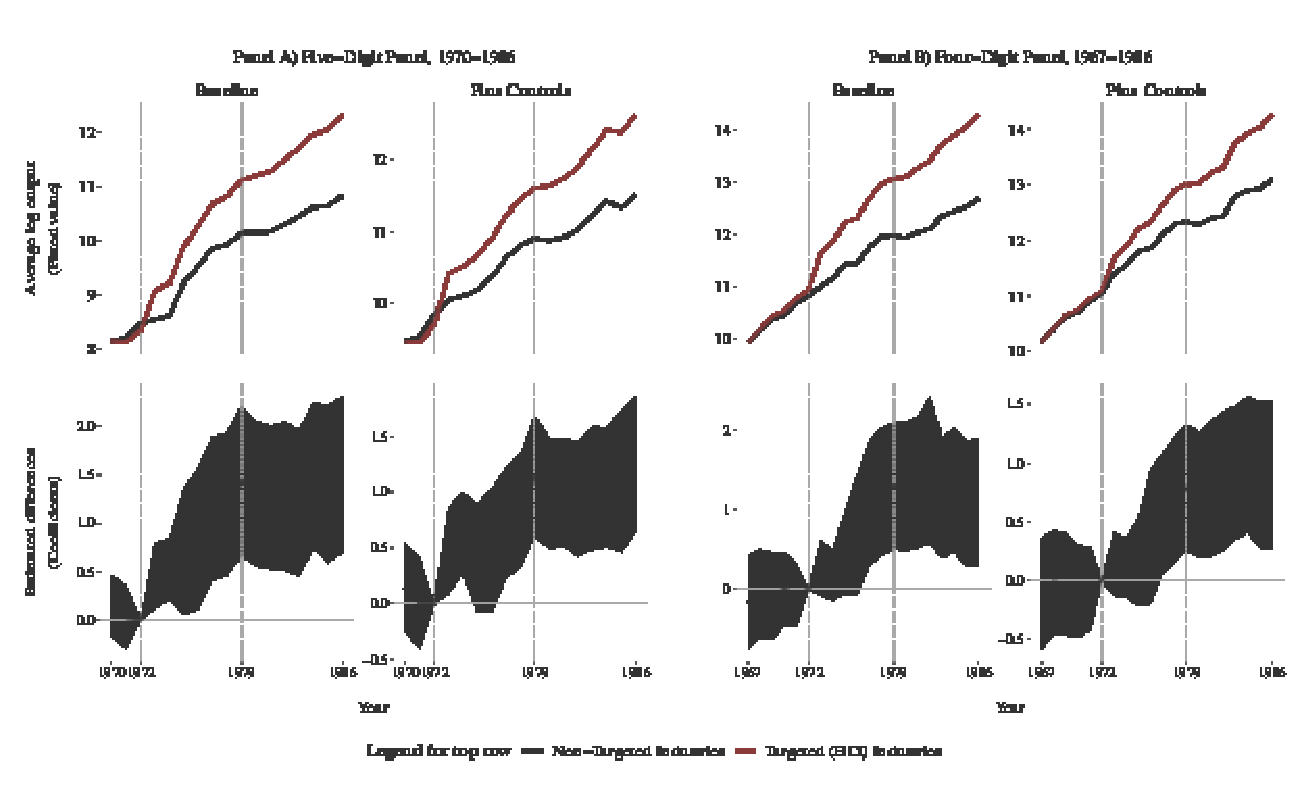
\includegraphics[scale=0.75]{Lane_QJE}
\par\end{centering}
\noindent\begin{minipage}[t]{1\columnwidth}%
\begin{singlespace}
{\small Source: \textcite{lane2025}. This figure presents dynamic
difference-in-differences estimates of the impact of HCI on output,
measured as the (log) real value of gross output shipped. The bottom
row displays DD estimates: Panel A for detailed 5-digit industries,
Panel B for aggregated 4-digit industries. ‘Baseline’ columns use
two-way fixed effects; ‘Plus Controls’ columns add pre-treatment controls.
The top row shows model-predicted outcomes, illustrating trends for
treated and control groups before and after 1972. All estimates are
relative to 1972, prior to the HCI policy. The year 1979 marks the
end of the Park regime. 95\% confidence intervals are shown in gray.}
\end{singlespace}
%
\end{minipage}
\end{figure}

\textcite{choi2025industrialization} leverage the timing of the HCI
policy and its regional variation, as the policy targeted the southeastern
part of the country. Their research design compares the difference
between firms in the HCI and non-HCI sectors in the targeted regions
to the difference in the non-targeted regions. The authors construct
a panel of firm-level policy interventions and balance sheets spanning
40 years, and employ a long-difference regression model to estimate
how much subsidized credit increased firm sales growth. The paper
has two appealing futures: First, it uses the post-double-selection
LASSO method to account for spillovers, addressing concerns about
SUTVA violation. Second, the paper uses a structural model of the
economy to translate local policy effects to aggregate welfare effect.
The empirical results show that subsidized firms grew faster than
those never subsidized for 30 years after subsidies ended. The quantitative
results imply that had the government not conducted this industrial
policy, welfare would have been 3-4\% lower. Most of the total welfare
effect (60-75\%) is due to the long-run impact of subsidies on productivity
through learning-by-doing (LBD). These findings again paint a positive
picture of the HCI drive. Additionally, the model-based counterfactual
simulation addresses some of the previously discussed limitations
of mere event studies.

\textcite{kim2021plant} paint a more nuanced picture the HCI drive's
impacts. The leverage \emph{plant-level} data to provide a more granular
view of how the policy affected productivity and resource allocation.
They show that manufacturing plants in the targeted industries (particularly
those in regions prioritized by the government) experienced much faster
growth in output and input usage than those in non-targeted industries
or regions. Labor productivity (output per worker) of targeted segments
also rose significantly relative to controls. Plant-level total factor
productivity (TFP) improved within targeted industry-region cells,
indicating technological progress at the establishment level. However,
the authors document a downside: the misallocation of resources \emph{within}
the targeted sectors worsened. In particular, many new entrant plants
in the favored industries were inefficient, causing a wider dispersion
of productivity and reducing the allocative efficiency in those sectors.
As a result, despite higher TFP at the micro (plant) level, the aggregate
TFP for the heavy industry sectors (when summing across plants) did
not increase more than in non-targeted sectors once resource misallocation
is accounted for.

\subsubsection*{Industrial Policy in China: Shipbuilding, Solar, and Decentralized
Competition}

China’s industrial policy has been evolving for years, with the “Made
in China 2025” initiative, launched in 2015, standing out prominently.
This ambitious plan seeks to position the country as a global leader
in high-tech manufacturing, particularly in sectors such as robotics,
aerospace, and electric vehicles. Recent academic studies have examined
various facets of China’s industrial policy---some focusing on specific
episodes, like subsidies in the shipbuilding and solar PV industries,
while others take a broader approach, assessing the overall economic
impact of these policies.

\textcite{barwick2025} study China’s 2006--2013 shipbuilding policy
using a dynamic structural model. The policy, worth RMB 634 billion
in subsidies, mixed production, investment, entry, and consolidation
measures. By fitting their model to pre-policy data and running counterfactual
simulations, they show that domestic investment surged by about 140\%,
firm entry by 120\%, and China’s global market share increased by
40\%. Notably, 70\% of this growth came at the expense of competitors
like Japan and South Korea. However, it is uncertain whether this
policy improved overall welfare, as it diverted limited resources
from other sectors of China’s economy. Without insights into the VMPL
differentials between alternative uses, the net welfare impact remains
ambiguous.

\textcite{banares2023ray} examine China’s solar PV policy, where
central and local governments backed solar panel makers with large
R\&D subsidies, feed-in tariffs, and export support. Using a synthetic
differences-in-differences approach, they find that Chinese cities
that implemented local solar policies experienced substantial and
enduring advantages, with solar manufacturer patent filings increasing
by over 50\% annually. The type of subsidy also mattered, as production
subsidies, particularly when paired with innovation subsidies, significantly
boosted the number of solar manufacturers, their total revenue, and
solar panel production. In contrast, demand subsidies had little impact
on local output and innovation, as additional demand was largely obtained
from other Chinese cities. Overall, revenue increased by RMB 135 million
(about US \$19 million), which is about 4.4 times the costs of the
policy. However, these findings do not provide clear insights into
net welfare effects, as measuring these requires accounting for revenue
losses in other industries or activities due to resource reallocation.
At best, one can claim that the policy delivered unambiguous welfare
gains through emissions reduction.

On a different note, \textcite{wang2025policy} analyze over 6,000
local policy pilots in China since 1980 to explore how decentralized
policy experiments affect outcomes. Their findings show that more
than 80\% of pilots were launched in wealthier areas where success
was more likely, with local officials pouring extra resources into
these tests---a boost that cannot be replicated nationally. As a
result, policies that shone in pilot conditions often fell short when
scaled up. Relatedly, \textcite{chen2021notching} identify another
limitation of industrial policy in the context of China’s InnoCom
program, which offers substantial tax cuts to firms that invest in
R\&D. Their analysis shows that many firms reclassified non-R\&D expenses
as R\&D to qualify for the incentives, leading to inflated R\&D reporting
without a corresponding rise in genuine innovative activity. These
findings challenge the broader literature that often portrays industrial
policy as having a positive impact on R\&D.”

\textcite{ju2024trade} provide a more holistic view of China's industrial
policy by examining the Made in China 2025 (MIC 2025) initiative.
Using a structural general equilibrium trade model with scale economies,
they assess the welfare impacts of MIC 2025 subsidies. Their findings
indicate that observed industrial subsidies increase with the degree
of scale economies, suggesting that these subsidies were well-targeted.
Furthermore, the subsidies benefit both the U.S. and China: they result
in a 2.47\% increase in China’s welfare by enhancing allocative efficiency
and a 0.44\% increase in U.S. welfare through positive spillovers,
primarily driven by a decline in intermediate input prices.

\subsubsection*{Industrial Policy in Advanced Economies}

Modern industrial policies in advanced economies increasingly reflect
environmental and geopolitical considerations. A leading example is
the United States’ Inflation Reduction Act (IRA) of 2022. The IRA
combines tax incentives and direct public expenditures to promote
the adoption and development of “green” technologies. \textcite{allcot2024ev}
examine the electric vehicle (EV) tax credits within the IRA framework
and conclude that, although the net social benefits are positive,
they remain modest relative to the program’s cost. Their findings
suggest that tailoring subsidies to account for variations in externalities
across vehicle types could yield significantly greater policy effectiveness.
Similarly, the U.S. CHIPS and Science Act of 2022 and the European
Chips Act of 2023 are aimed at bolstering domestic semiconductor manufacturing
capacity, an area of strategic importance. \textcite{goldberg2024semiconductor}
document a marked increase in government intervention in the semiconductor
sector since 2020 across several major economies, including China,
the U.S., Japan, Korea, and India. Taiwan, which produces approximately
60\% of the world’s semiconductors, notably remains an exception.
The study finds that while learning-by-doing effects are present,
they are smaller than commonly assumed. In contrast, international
spillovers from these policies are sizable.

Empirical research has also explored historical policy episodes, suggesting
possibly long-lasting influence on industrial trajectories. During
the late 19th century, British shipyards benefited from early adoption
of metal shipbuilding and relatively lower iron input prices, which
presented a significant cost advantage over North American rivals.
Although iron prices began to converge in the 1890s following new
discoveries in the U.S., British dominance persisted. \textcite{hanlon2020shipbuilding}
finds that while British producers maintained their leadership even
after their cost advantage eroded, North American firms operating
in regions with less direct British competition were more successful
in transitioning from wooden to metal ships. Establishing the causal
effects of initial advantage is, however, difficult. \textcite{juhasz2018infant}
addresses this challenge through a natural experiment to test the
infant industry hypothesis in the context of early 19th-century cotton
industry mechanization. During the Napoleonic Wars (1803--1815),
the Continental Blockade curtailed the entry of British goods into
continental Europe, affording French firms temporary trade protection.
This shock accelerated the adoption of mechanized cotton-spinning
technology in affected regions, with measurable effects persisting
decades beyond the blockade. The study overcomes the endogeneity typically
associated with industrial policy evaluation by leveraging an exogenous
shock---independent of policymaker discretion. Nonetheless, this
methodological strength limits the paper’s direct applicability to
current policy design, as it does not assess whether \emph{targeted}
support for mechanization improves allocative efficiency.

\textcite{km2013tva} explore the long-term impacts of place-based
industrial policy through the lens of the Tennessee Valley Authority
Act of 1933, a cornerstone of President Franklin D. Roosevelt’s New
Deal. The Act created the TVA and invested heavily in regional infrastructure
to spur agricultural and industrial development. To address selection
bias in evaluating TVA’s impact, the authors use \emph{proposed but
never approved} ``valley authority'' bills to construct comparison
groups. Their findings show that the TVA boosted regional manufacturing
employment, with effects persisting well after subsidies ended. However,
from a national perspective, the local gains were likely offset by
employment losses in other parts of the country, highlighting the
redistributive nature of such interventions. These national-level
effects are estimated using a structural model designed to isolate
labor market effects, but may fail to capture other general equilibrium
changes that are relevant to welfare.

In the United Kingdom, the Industrial Development Act of 1982 introduced
the Regional Selective Assistance (RSA) program, offering discretionary
grants to firms in economically disadvantaged areas. The program covered
up to 35\% of investment costs for projects meeting specific job creation
thresholds. \textcite{criscuolo2019RSA} evaluate the program’s effectiveness
by exploiting shifts in EU-defined eligibility criteria during the
UK’s membership. The paper finds that the policy increases manufacturing
employment, reduces aggregate unemployment, and that the effects are
not purely due to the relocation of jobs from eligible to ineligible
areas. The positive effects, however, exist only for small firms,
while large companies accept subsidies without increasing activity.
The paper similarly does not find evidence in support of the ``big
push'' hypothesis.\footnote{Beyond the context of Korea, China, and Advanced economies, \textcite{manelici2021industrial}
study Romania’s 2001 personal income tax break for IT workers and
its 2013 expansion. They find that the policy led to sustained firm-level
growth, sectoral expansion relative to similar countries, and positive
spillovers to downstream sectors relying on IT inputs.}

\subsection*{Ex Ante Measurement of Optimal Policy Outcomes}

The studies reviewed earlier examine the local effects of past industrial
policies, which are often small-scale interventions conducted in a
specific context. While learning from these successes and failures
can shed light on the overall effectiveness of such policies, it is
important to recognize the challenges in drawing clear conclusions
from such data. Past failures might stem from limited scope or poor
targeting, which does not necessarily mean similar policies would
fail in different contexts. Therefore, policymakers might not be deterred
from implementing comparable strategies in the future despite the
evidence, nor gain substantial insights into crafting more effective
policies in other contexts.

A newer approach tackles these issues differently. It combines theoretical
frameworks with empirical data to map out the \emph{ex ante }potential
of industrial policies across various countries. By identifying the
best possible outcomes, this method can offer more actionable guidance
to policymakers. For example, if even an optimally designed import
substitution policy yields limited benefits, it strengthens the argument
against its implementation.

Before discussing the inherent limitations of the ex ante approach
and reviewing existing work, it is useful to compare this approach
with the ex post studies from a purely methodological standpoint.
Both can be viewed as variants of the ``potential outcomes'' framework.
In ex post analyses, researchers use the policy’s design to divide
economic units into comparable treatment and control groups, and infer
potential outcomes under different treatment conditions, i.e., the
Rubin causal model. In contrast, the ex ante approach is a model-based
approach for determining potential outcomes under counterfactual policy:
researchers estimate supply and demand elasticities, interpret them
structurally, and then use these models to predict outcomes under
hypothetical scenarios set by a central planner.

Figure \ref{fig:Ex-ante-model-based} presents a highly stylized depiction
of the model-based approach for simulating policy counterfactuals.
The process begins with observed data, such as quantities and their
associated tax rates---as shown in the left panel. For illustrative
purposes, assume that each data point corresponds to a distinct point
in time, with the current observation indicated by the solid blue
marker. A central assumption is that these data are generated by a
micro-founded structural model, where the elasticity of quantity with
respect to taxation, $\epsilon$, is constant and structural in nature.
Given the structural relationship represented by the red fitted line,
the researcher can simulate the effects of a hypothetical optimal
policy reform, $\Delta\ln\tau^{*}$, on equilibrium quantities, $\Delta\ln q^{*}$,
and then, using the underlying utility function, translate these quantity
changes into an associated welfare effect, $\Delta\ln W^{*}$.\footnote{In the context of trade models, this approach is referred to as the
exact hat algebra method. \textcite{baqaee2024networks} demonstrate
that the assumption of constant elasticity, $\epsilon$, can be partially
relaxed through a step-wise implementation of hat algebra. Furthermore,
\textcite{dingel2020spatial} underscore key limitations of this method
in granular settings, particularly when matrices representing bilateral
flows are sparse.} Although the figure abstracts from many of the empirical complexities
inherent in contemporary quantitative models, it effectively conveys
the core logic underpinning the ex ante approach reviewed in this
section.

\begin{figure}[!tbh]
\caption{Model-based approach for predicting ex ante optimal policy outcomes }\label{fig:Ex-ante-model-based}

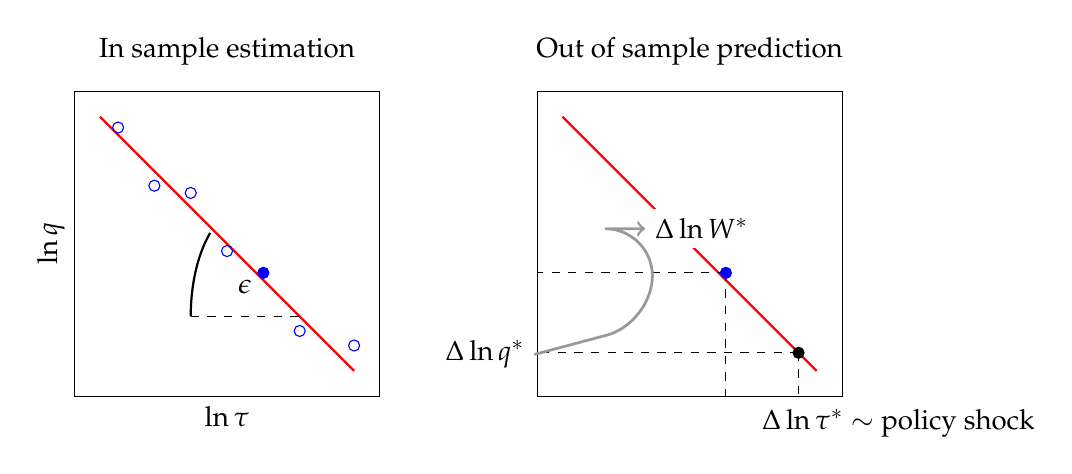
\begin{tikzpicture}[scale=1.0]

  % Left plot
  \begin{axis}[
      name=left,
      width=0.45\textwidth,
      height=0.45\textwidth,
      xlabel={$\ln \tau$},
      ylabel={$\ln q$},
      title={In sample estimation},
      grid=both,
      clip=false,
	  xtick=\empty,
      ytick=\empty]  % Important to ensure nothing gets clipped away
    % Scatter points
    \addplot[only marks, mark=o, blue] coordinates {
      (0.1, 3.01)
      (0.2, 2.93)
      (0.3, 2.92)
      (0.4, 2.84)
	  (0.6, 2.73)
      (0.75, 2.71)	
    };
	\addplot[only marks, mark=*, blue] coordinates {(0.5, 2.81)};

    % Fitted line
    \addplot[domain=0.05:0.75, red, thick] { -0.5*x + 3.05 };

    % Horizontal dashed line
    \draw[dashed] (axis cs:0.3,2.75) -- (axis cs:0.6,2.75);

    % Label
    \node at (axis cs:0.45,2.79) {$\epsilon$};

    % Parametric arc near (0.45,2.79).
    % This draws a short curve for angles 180 to 150 around that center.
    \addplot [
      thick,
      black,
      domain=180:130,
      samples=20
    ] (
      {0.45 + 0.15*cos(x)},
      {2.75 + 0.15*sin(x)}
    );

  \end{axis}

  % Right plot
  \begin{axis}[
      name=right,
      at={(left.east)},
      anchor=west,
      xshift=2cm,
      width=0.45\textwidth,
      height=0.45\textwidth,
      title={Out of sample prediction},
      grid=both,
	  xtick=\empty,
      ytick=\empty]
    % Fitted line
    \addplot[domain=0.05:0.75, red, thick] { -0.5*x + 3.05 };

    % Original equilibrium point
    \addplot[only marks, mark=*, blue] coordinates {(0.5, 2.81)};

    % Counterfactual tariff
    \addplot[only marks, mark=*, black] coordinates {(0.7, 2.7)};

    % Dashed line connecting points
    \draw[dashed] (axis cs:0.5,2.81) -- (axis cs:0.5,0);
    \draw[dashed] (axis cs:0.7,2.7) -- (axis cs:0.7,0);
	
	\draw[dashed] (axis cs:0.5,2.81) -- (axis cs:-0.1,2.81);
    \draw[dashed] (axis cs:0.7,2.7) -- (axis cs:-0.1,2.7);
    
    

    % Arrow to welfare calculation
    %\draw[->, dashed] (axis cs:0.7,2.7) -- (0.6,3);

    % Text box
    %\node[anchor=west] at (axis cs:0.6,3.0) {cccc};

  \end{axis}

  \node[anchor=north] at ($(right.south) + (2.65,-1pt)$) {$\Delta \ln \tau^{*} \sim $ policy shock};
  \node[anchor=east] (deltaq) at ($(right.west) + (-1pt,-40pt)$) {$\Delta \ln q^{*}$};

  \node[anchor=south west, fill=white] (welfare) at ($(right.north east) + (-25mm,-20mm)$) {$\Delta \ln W^{*}$};
   \draw[->, rounded corners=6mm, line width=1pt, draw=gray!80] 
    (deltaq.east) -- ++(1.5cm,0.4) coordinate (A) 
    -- (A |- welfare.west) -- (welfare.west);

\end{tikzpicture}

\noindent\begin{minipage}[t]{1\columnwidth}%
\begin{singlespace}
{\footnotesize\emph{Note}}{\footnotesize : This stylized illustration
depicts the ex ante model-based methodology for simulating counterfactual
policy effects. The left panel shows an example of data points on
quantities and tax rates, with the current state of the economy marked
by the solid blue marker. Under the assumption that data are generated
by a structural model with constant elasticity $\epsilon$ (red fitted
line), researchers can simulate the effects of an optimal policy reform
($\Delta\ln\tau^{*}$) on equilibrium quantities ($\Delta\ln q^{*}$)
and translate these into welfare effects ($\Delta\ln W^{*}$) using
the underlying utility function consistent with constant elasticity
assumption. }
\end{singlespace}
%
\end{minipage}
\end{figure}

A key limitation of the model-based approach is that its predictions
are only as reliable as the model itself. Models can be misspecified
for several reasons. First, it is virtually impossible to account
for all possible economic distortions without losing tractability,
so models typically focus on a single distortion. Recent work by \textcite{adao2024putting}
has made notable progress in externally validating quantitative models.
Second, accurately estimating a designated distortion requires overcoming
well known identification challenges. Lastly, since these are aggregate,
multi-regional models calibrated to broad data, they cannot easily
accommodate firm-level distortions or assess interventions that target
level individual firms. Instead, the ex ante approach is more suited
for examining traditional industrial policies that involve reallocating
resources across broadly defined sectors or industries. With these
caveats in mind we know review the relevant literature.

\subsubsection*{The Gains from Efficient Industrial Policies}

The literature on optimal industrial policy has a long and rich tradition,
though it remains predominantly theoretical. A prominent recent contribution
is \textcite{itskhoki2019optimal}, who characterize optimal industrial
policy in the presence of financial frictions. In parallel, a substantial
body of research has focused on quantifying the welfare costs of misallocation
(e.g., \cite{hsieh2009misallocation,restuccia2008policy,restuccia2013misallocation,bai2024misallocation}),
which indirectly highlights the potential welfare gains from optimal
policy interventions. Nonetheless, explicit analyses of optimal and
constrained-optimal industrial policy remain relatively limited. Much
of the existing work in this area is grounded in quantitative trade
and spatial models and leverages the exact hat-algebra method for
counterfactual policy simulations (\cite{dekle2008global}).

Several papers have explored the the gains from optimal place-based
policies. \textcite{fajgelbaum2020optimal} analyze optimal spatial
policies in the U.S. that include place-based taxes and interregional
transfers. Their framework feature local agglomeration economies and
distinguishes between low- and high-skill workers. Based on their
analysis, optimal policy yields approximately 4\% welfare gains for
all workers, and requires additional transfers from high- to low-wage
locations compared to observed patterns. Essentially their analysis
reveals that larger U.S. metropolitan areas are overly populated,
particularly with high-skill workers. Optimal allocation, thus, shifts
high-skill workers toward smaller, skill-scarce cities where they
have a higher VMPL. Relatedly, \textcite{rossi2019cognitive} study
optimal redistribution with worker heterogeneity, motivated by increasing
spatial polarization of cognitive occupations within U.S. urban centers.
Their model distinguishes industries by cognitive occupation intensity
and estimates agglomerate externalities that vary with city size and
composition. Cognitive workers experience positive within-group externalities
but negative effects from other groups. The optimal spatial allocation,
in their model, asks for increased concentration of cognitive workers
in major hubs than current levels. The overall gain in welfare from
optimal policy is more modest in their analysis, amounting to 0.72\%
percent of GDP. 

A couple of trade paper examine industrial policy effects in its more
traditional definition. \textcite{lashkaripour2023profits} use a
quantitative trade model with industry-level external economies of
scale. In their setup, external economies emerge from firm entry and
love for variety. Specifically, the distortion wedge in their analysis
corresponds to the scale elasticity, $\psi_{i}$, and market power,
$(\mu_{i}-1)/\mu_{i}$, as defined in the earlier sections. They estimate
$\psi_{i}$ by measuring the extent of consumers’ taste for variety,
using high-frequency transaction-level data that allows identifying
the firm-level demand curvature. The estimated curvature directly
reveals the degree of love for variety within each industry. An important
aspect of their method is separately identifying the trade elasticity,
$\epsilon_{i}$, from the scale elasticity, $\psi_{i}$, for each
industry. This distinction is crucial for credible policy analysis,
as emphasized under Remark 4.

Employing global data on industry-level expenditure, trade, and employment
shares, along with their jointly estimated scale and trade elasticities,
the authors calculate potential gains from implementing globally optimal
industrial policies---policies that correct scale distortions universally
(Equation \ref{eq: optimal policy (global)}). They conclude that
real GDP would rise by an average of 3.4 percent across the countries
in their sample. For countries such as Indonesia and Mexico, these
benefits are especially significant, exceeding 6 percent. These substantial
gains reflect large variation in scale elasticities across industries.
Following \textcite{ding2024global}, the gains from efficient policy
are equal to average Bergman distance between scale elasticities and
their mean with generating function $f\left(\psi\right)=\psi\ln\left(1+\psi\right)$,
which is approximately equal to variance of the scale elasticities
for sufficiently small elasticity values. More specifically, the welfare
change from implementing the optimal subsidy $\tau_{i}^{*}=\psi_{i}^{*}$
is
\[
\Delta\ln W=\mathbb{E}_{\beta}\left[\psi_{i}\ln(1+\psi_{i})\right]-\mathbb{E}_{\beta}\left[\psi_{i}\right]\ln\mathbb{E}_{\beta}\left[1+\psi_{i}\right]\approx\text{Var}_{\beta}\left[\psi_{i}\right],
\]
where $\mathbb{E}_{\beta}\left[z_{i}\right]=\sum_{i}\beta_{i}z_{i}$
is the expenditure weighted mean operator.

\textcite{BCDR} conduct a similar analysis, albeit employing a different
methodology for estimating scale elasticities. Their approach begins
by inferring region-specific industry-level price indexes from trade
volume data, which are then regressed on employment size to identify
the scale elasticities. Compared to the previous paper, this method
captures scale elasticity in a broader sense but relies on externally
estimated trade elasticities to for the identification of price indexes.
This dependence is inconsequential when evaluating the gains from
first-best policies, but it has implications for the gains from unilaterally-adopted
policies. In such cases, as previously discussed, the interplay between
scale and trade elasticities significantly shapes policy outcomes.
Overall, \textcite{BCDR} estimate smaller and less heterogeneous
scale elasticities, leading to more modest gains from optimal (first-best)
subsidies---approximately 1.1\% for the average country. However,
when input-output linkages are incorporated, the estimated gains increase
substantially, exceeding 4\% on average.

A central result in \textcite{BCDR} is that small economies with
high trade-to-GDP ratios are especially well positioned to gain from
industrial policy. The mechanism is straightforward. When subsidies
induce labor to move from low- to high-VMPL sectors, the welfare gain
rises with the size of this reallocation. In their model, the extent
of reallocation is limited by imperfect substitutability across sectors.
In small open economies, however, inelastic domestic demand is less
of a constraint, so the policy induced reallocation is larger, and
so are the welfare gains.\footnote{This conclusion appears at odds with \textcite{lashkaripour2023profits},
harking back to tension outlined under Remark 4. In \textcite{lashkaripour2023profits},
trade openness has two opposing effects on optimal policy gains: a
positive one, as in \textcite{BCDR}, and a negative one, arising
because scale and trade elasticities are negatively correlated across
sectors. The different conclusions, thus, stem from the different
estimation strategies. \textcite{lashkaripour2023profits} jointly
estimate the trade and scale elasticities, identifying a negative
correlation. \textcite{BCDR}, by contrast, estimate scale elasticities
using price indexes constructed from externally estimated trade elasticities.
Their approach is not well suited to identify the correlation between
scale and trade elasticities, which drives the negative effect. However,
their estimation of inter-sectoral substitutability makes their model
better suited to quantify the positive effect of openness.}

\subsubsection*{The Effectiveness of Second-Best Industrial Policies}

In practice, industrial policies often have limited scope and are
imprecisely targeted. Several studies have quantified the potential
gains from industrial policy under second-best conditions---scenarios
in which governments concentrate their efforts on a narrow range of
industries or regions, or employ indirect, poorly-targeted interventions.
For instance, rather than offering direct subsidies, policymakers
may seek to stimulate domestic industrial output by restricting imports
or encouraging exports. In some cases, these trade-based measures
are optimal, particularly when inefficient export barriers prevent
industries from achieving an efficient scale, as reviewed by \textcite{reed2024export}.
Yet, more often, such instruments are chosen simply because they are
politically more feasible to implement (\cite{rickard2025tariffs}).

In this context, \textcite{lashkaripour2023profits} evaluate the
effectiveness of trade policies, specifically import substitution
and export promotion, as instruments of industrial policy. Surprisingly,
they find trade measures quite ineffective at addressing sectoral
misallocations caused by scale economies or market power. Even under
optimal design, trade policies realize less than one-third of the
potential gains achievable with direct subsidies. Two key reasons
drive this result. First, trade policies inherently lack precision.
Optimal resource allocation requires targeted subsidies, whereas trade-based
instruments can only partially mimic the optimal subsidies, as noted
under Remark 3. Second, trade policies inherently distort international
prices, undermining overall trade efficiency. Earlier in this essay
we discussed circumstances where correcting scale distortions diminishes
the efficiency gains from trade. Thus, the optimal second-best policy,
by necessity, balances these competing efficiency considerations,
making it ultimately inferior to precisely targeted subsides. \textcite{antras2024trade}
report similar limitations for second-best trade policies compared
to unilaterally optimal trade and production taxes, using scale elasticity
estimates from \textcite{BCDR}.

\textcite{liu2019network} examines a scenario in which governments,
operating with limited fiscal resources or policy instruments, aim
to support industries offering the greatest marginal value of public
funds (MVPF). Echoing the logic outlined earlier in this essay, \textcite{liu2019network}
demonstrates that the MVPF associated with subsidies to a given industry
corresponds to that industry’s distortion centrality---defined as
its distortion divided by the Domar weight. Furthermore, if the government
is constrained to providing only value-added subsidies, the constrained-optimal
subsidies are proportional to distortion centrality. These findings
offer an \emph{ex ante} benchmark for ranking incremental industrial
policy reforms. The author then applies this theoretical framework
to perform ex post evaluation of South Korea's 1970s and China's contemporary
industrial policy. In both cases, policies align with theoretical
benchmark, targeting industries that exhibit high distortion centrality---heavy
manufacturing in South Korea and strategic sectors in today’s China.
Policy simulations indicate that China’s industrial policies, taken
together, raised overall economic efficiency by 6.7 percent.

How, then, can we reconcile \citeauthor{liu2019network}'s \parencite*{liu2019network}
conclusions with the limited gains from optimal policy implied by
the quantitative trade models reviewed previously? First and foremost,
Liu assumes that distortion wedges (like monopolistic markups) create
quasi-rents that vanish from the economy as pure deadweight loss.
By contrast, in the closest comparable scenario, \textcite{lashkaripour2023profits}
model these rents as profits retained within the economy and returned
to consumers. Consequently, Liu’s treatment of wedges inherently exaggerates
the magnitude of deadweight losses. Another key difference lies in
scope: Liu’s analysis operates at a more granular level, identifying
distortions at the individual-firm level rather than across entire
industries. This is made possible by Liu's focus on one country. Finally,
and importantly, Liu’s model treats China as a closed economy. This
assumption excludes the trade-related tensions that diminish optimal
policy gains.\footnote{\textcite{liu2019network} explores an open economy adjustment in
which a fictitious “trade intermediary” sector sells imports and purchases
exports, operating under constant returns to scale. This stylized
setup naturally avoids the tensions examined in this paper, which
occur when each sector is directly traded.}

\subsubsection*{The Importance of Regional or International Policy Coordination}

In the 2024 \emph{Draghi report on EU competitivenes}, policy coordination
is discussed more than 100 times. Draghi, in his speech to the European
Union (EU), highlighted poor coordination between member states as
a major weakness. In line with these concerns, several academic studies
examine industrial policy coordination. Some studies address coordination
between countries, while others investigate internal coordination
among regional governments.

At an international level, \textcite{lashkaripour2023profits} argue
that when national governments commit to shallow integration, as in
the EU system, industrial policy coordination becomes more vital.
Unilateral policy adoption under free trade leads to strong positive
spillovers to trading partners, but can worsen the home country's
terms of trade to the point of causing immizerising growth effects.
They proceed to quantify these effects by simulating policy outcomes
under coordinated and unilaterally-adopted corrective policies: $\tau_{i}^{*}=\phi_{i}$.
The results displayed in Table \ref{tab:Policy coordination} show
that unilateral corrective subsidies surprisingly lead to economic
losses for the average country. This occurs because negative terms
of trade effects outweigh the benefits from correcting scale or markup
distortions.

\begin{table}[!tbh]
\caption{Importance of Policy Coordination}\label{tab:Policy coordination}

\begin{tabular}{lccccccc}  \toprule &&    \multicolumn{2}{c}{Market power distortions}   & \phantom{abc} &   \multicolumn{2}{c}{Scale distortions}  \\  \cmidrule{3-4}    \cmidrule{6-7} &&          \specialcell{Unilateral} &  \specialcell{Coordinated}  && \specialcell{Unilateral} &  \specialcell{Coordinated}  \\  
\midrule 
\specialcell{Gains from \emph{corrective} \\  industrial policy ($\tau_{i}^{*}=\phi_{i}$)} && -0.32\% & 1.67\% && -2.78\% & 3.42\%  \vspace{0.05in} \\ 
\bottomrule 
\end{tabular} 
\vspace*{0.01in}\\
\noindent\begin{minipage}[t]{1\columnwidth}%
\begin{spacing}{0.8}
{\footnotesize Sourc}{\small e: \textcite{lashkaripour2023profits}.
This table reports the gains from implementing efficient subsidies
in a unilateral versus coordinated manner. Under market power distortions,
the efficient subsidy is equal to excess markup, $\tau_{i}^{*}=(\mu_{i}-1)/\mu_{i}$.
Under scale distortions the optimal policy is a subsidy equal to the
scale elasticity $\tau_{i}^{*}=\psi_{i}$. The report welfare effects
are averages across all countries in the sample.}
\end{spacing}
%
\end{minipage}
\end{table}

In a related study, \textcite{hodge2024industrial} simulate industrial
policy outcomes for the EU and reach similar conclusions. They argue
that unilateral industrial policies can harm domestic welfare by causing
unfavorable production relocation and terms of trade effects, particularly
in smaller, open economies. Coordinating industrial policies within
the EU and with politically-aligned non-EU countries proves beneficial
for all involved, reducing negative spillovers and yielding higher
welfare gains by preventing production relocation and negative trade
effects. They highlight Airbus as a successful example of cross-border
policy coordination, whereas Germany’s solar industry illustrates
the difficulties of acting unilaterally.

In a domestic context, \textcite{ferrari2023quantitative} study the
costs of non-cooperative industrial policies among regional governments
in the U.S. They measure the economic losses resulting from a non-cooperative
Nash equilibrium involving state-level subsidies. Their results show
states have significant incentives to use subsidies to attract businesses,
typically harming other states. On average, optimal subsidies reach
\$14.9 billion, increasing real income by 2.2 percent in the subsidizing
state but causing a 0.2 percent decrease in other regions. Notably,
currently-applied subsidies resemble cooperative outcomes more closely
than purely non-cooperative ones. Yet, stronger subsidy competition
could be harmful: moving from current subsidy levels to a Nash equilibrium
would reduce real income by 1.1 percent, while shifting to fully cooperative
(zero-subsidy) policies would yield only slight welfare gains.

\section*{Concluding Remarks and Directions for Future Research}

The resurgence of industrial policy in the face of global challenges,
ranging from climate change to geopolitics, has prompted renewed interest
in its theoretical and empirical foundations. This essay revisited
the rationale for industrial policy in the presence of various market
failures, with particular attention to defining characteristics of
modern economies, including complex input-output linkages and high
levels of trade integration.

A key takeaway from the theoretical framework is that, irrespective
of underlying economic complexities, optimal policy is merely a targeted
subsidy that removes the distortion wedge. Yet the resulting welfare
gains are amplified when targeted industries are more central in the
production network or face more elastic demand. In practice, however,
policy implementation is often limited in scope and may resort to
trade instruments as a second-best policy. These indirect interventions
carry inherent limitations, especially in open economies, where they
can produce adverse international spillovers or transfer income from
domestic households to foreign entities.

Empirical evidence on past industrial policies paint a nuanced picture.
Some cases, such as South Korea’s HCI drive point to lasting benefits
driven by productivity gains and learning-by-doing. However, several
studies reveal unintended consequences and modest returns once spillovers
and general equilibrium effects are taken into account. China’s recent
industrial policy efforts highlight both the advantages of targeted
support and the challenges of scaling up from decentralized policy
trails. Meanwhile, advanced economies are increasingly employing industrial
policy to pursue geopolitical and environmental objectives. However,
the long-term effectiveness of these efforts remains uncertain, as
they involve uncharted goals and are being implemented under largely
untested economic conditions.

Complementing the empirical approach, forward-looking model-based
evaluations provide insights on the potential gains from optimally-designed
interventions. These analyses suggest that while efficient industrial
policies can yield notable welfare improvements, they are barely transformative.
In practice, however, governments seldom implement precisely targeted
subsidies. Instead, they often rely on second-best instruments, which
tend to perform poorly, even under optimal design. An additional layer
of complexity arises from growing trade openness. As trade integration
deepens, even carefully targeted unilateral policies risk generating
welfare losses due to adverse terms-of-trade effects, reinforcing
the importance of international policy coordination.

In sum, the effectiveness of industrial policy depends on its design,
the precision with which it targets distortions, and the degree of
coordination achieved across regions. Recent advances in both theoretical
frameworks and empirical methodologies have deepened our understanding
of the conditions under which such policies can improve economic welfare.
Nevertheless, many uncertainties remain. In particular, there is limited
work on the optimal design of industrial policies when technology
adoption itself is shaped by policy. Although a growing body of literature
identifies inefficient technology choices as a primary source of misallocation
in developing economies (e.g., \cite{farrokhi2024trade,dix2021trade}),
there has been surprisingly limited exploration of how industrial
interventions might remedy these inefficiencies.

On a broader level, \textcite{rodrik2009industrial} argues that debates
over industrial policy \emph{``are rarely ever about whether the
government should be involved; they are about how the government should
go about running its policies.''} He outlines three principles for
improving \emph{how} policy is executed: first, \emph{embeddedness},
which entails close collaboration between policymakers and industry
experts to ensure grounded decision-making; second, \emph{discipline},
which requires clear objectives, rigorous evaluation processes, and
the timely discontinuation of funds to underperforming units; and
third, \emph{accountability}, to ensure that policymakers are liable
for outcomes. Among these, the role of embeddedness offers particularly
fertile ground for future research. Early empirical studies involving
human expertise (\cite{fafchamps2017identifying,mckenzie2019predicting})
show limited success. However, combining expert judgment with advanced
machine learning techniques holds promise for better outcomes, as
shown in other domains (\cite{mullainathan2022diagnosing}). Further
exploration into this hybrid embeddedness approach presents a promising
path for future research.

\theendnotes

\printbibliography
\begin{refsection}
    \nocite{choi2025industrialization,lashkaripour2023profits,lane2025,barwick2025,liu2019network} 
    \printbibliography[title={Further Reading}]
\end{refsection}


\appendix

\section{Appendix: Welfare Derivations}

Per utility maximization implies, we can specify welfare using the
indirect utility function in terms of income and prices. In particular,
\[
C=v(\,Y\,,\,\{p_{i}^{\tau}\}_{i}\,),\qquad where\qquad p_{i}^{\tau}\equiv(1-\tau_{i})p_{i}
\]
where income $Y$ is the sum of wage income, profit payments, and
lump-sum tax rebates:
\[
Y=wL+\sum_{i}\pi_{i}-\sum_{i}\tau_{i}p_{i}q_{i}=wL+\sum_{i}(\frac{\mu_{i}-1}{\mu_{i}}-\tau_{i})p_{i}q_{i}
\]
Welfare is accordingly the difference between the indirect utility
from consumption and the disutility from environmental externalities:
\[
W=v(Y,\{\left(1-\tau_{i}\right)p_{i}\}_{i})-\sum_{i}\delta_{i}q_{i}
\]
 Taking derivatives from the welfare function specified above yields
\[
\frac{\partial W}{\partial(1-\tau_{j})}=\frac{\partial v(.)}{\partial Y}\frac{\partial Y}{\partial(1-\tau_{j})}+\sum_{i}\frac{\partial v(.)}{\partial p_{i}^{\tau}}\frac{\partial p_{i}^{\tau}}{\partial(1-\tau_{j})}-\sum_{i}\delta_{i}\frac{\partial q_{i}}{\partial(1-\tau_{j})}
\]
The change in welfare in response to policy $\tau_{j}$ starting from
the status quo ($\tau=0$). Taking derivatives w.r.t. income we get
\[
\frac{\partial Y}{\partial\left(1-\tau_{j}\right)}=p_{j}q_{j}+\sum_{i}(\frac{\mu_{i}-1}{\mu_{i}}-\tau_{i})\left[p_{i}\frac{\partial q_{i}}{\partial(1-\tau_{j})}+q_{i}\frac{\partial p_{i}}{\partial(1-\tau_{j})}\right].
\]
In the neighborhood of status quo, $\tau=0$, we get 
\[
\frac{\partial Y}{\partial\ln(1-\tau_{j})}=p_{j}q_{j}+\underbrace{\sum_{i}\frac{\mu_{i}-1}{\mu_{i}}\left[p_{i}\frac{\partial q_{i}}{\partial(1-\tau_{j})}+q_{i}\frac{\partial p_{i}}{\partial(1-\tau_{j})}\right]}_{\partial\pi/\partial(1-\tau_{j})}
\]
where $\omega_{j}\equiv p_{j}q_{j}/Y$ is the revenue-based Domar
weight. Next, consider the price effect
\[
\frac{\partial v(.)}{\partial p^{\tau}}\cdot\frac{\partial p_{}^{\tau}}{\partial\ln(1-\tau_{j})}=\sum_{i}\frac{\partial v(.)}{\partial p_{i}^{\tau}}\frac{\partial p_{i}^{\tau}}{\partial(1-\tau_{j})}=\frac{\partial v\left(.\right)}{\partial Y}\left\{ \sum_{i}c_{i}\frac{\partial\ln p_{i}^{\tau}}{\partial(1-\tau_{j})}\right\} 
\]
we can characterize 
\[
\frac{\partial\ln p_{i}^{\tau}}{\partial\ln(1-\tau_{j})}=1_{i=j}+\frac{\partial\ln p_{i}}{\partial\ln q_{i}}\frac{\partial\ln q_{i}}{\partial\ln(1-\tau_{j})}+\sum_{s}\frac{\partial\ln p_{i}}{\partial\ln p_{s}^{\tau}}\frac{\partial\ln p_{s}^{\tau}}{\partial\ln(1-\tau_{j})}
\]
Shephard's lemma implies that $\frac{\partial\ln p_{i}}{\partial\ln p_{s}^{\tau}}=\Omega_{si}$
, where $\Omega_{si}$ is the entry $\left(i,s\right)$ of the input-output
matrix. Plugging this into above equation, delivers
\[
\frac{\partial\ln p_{i}^{\tau}}{\partial\ln(1-\tau_{j})}=1_{i=j}-\psi_{i}\frac{\partial\ln q_{i}}{\partial\ln(1-\tau_{j})}+\sum_{s}\Omega_{si}\frac{\partial\ln p_{s}^{\tau}}{\partial\ln(1-\tau_{j})},
\]
which after rearranging and inverting yields the following, where
$\Psi_{is}$ is the entry $\left(i,s\right)$ of the Leontief inverse
matrix:
\[
\frac{\partial\ln p_{i}^{\tau}}{\partial\ln(1-\tau_{j})}=\sum_{s}\Psi_{si}\left[1_{s=j}-\psi_{s}\frac{\partial\ln q_{s}}{\partial\ln(1-\tau_{j})}\right]
\]
We can insert the above price equation into previously derived expressions
and 
\begin{align*}
\frac{\partial v(.)}{\partial p_{}^{\tau}}\cdot\frac{\partial p_{}^{\tau}}{\partial\ln(1-\tau_{j})} & =\frac{\partial v\left(.\right)}{\partial Y}\left\{ \sum_{i}p_{i}^{\tau}c_{i}\frac{\partial\ln p_{i}^{\tau}}{\partial\ln(1-\tau_{j})}\right\} \\
 & =-\frac{\partial v\left(.\right)}{\partial Y}\left\{ \sum_{i}\left[\Psi_{ij}p_{i}^{\tau}c_{i}\right]-\sum_{i}\sum_{s}\left[\Psi_{is}p_{s}^{\tau}c_{s}\right]\psi_{i}\frac{\partial\ln q_{i}}{\partial\ln(1-\tau_{j})}\right\} 
\end{align*}
Likewise for the effect on profits
\begin{align*}
\frac{\partial\pi}{\partial\ln(1-\tau_{j})} & =\sum_{i}\frac{\mu_{i}-1}{\mu_{i}}p_{i}q_{i}\left[\frac{\partial\ln q_{i}}{\partial\ln(1-\tau_{j})}+\frac{\partial\ln p_{i}}{\partial\ln(1-\tau_{j})}\right]\\
=\sum_{i} & \left[\frac{\mu_{i}-1}{\mu_{i}}p_{i}q_{i}-\sum_{s}\left[\Psi_{is}\frac{\mu_{s}-1}{\mu_{s}}p_{s}^{\tau}q_{s}\right]\psi_{i}\right]\frac{\partial\ln q_{i}}{\partial\ln(1-\tau_{j})}+\sum_{i}\frac{\mu_{i}-1}{\mu_{i}}\left(\Psi_{ji}-1_{i=j}\right)p_{i}q_{i}\\
 & =\sum_{i}\left(\frac{\mu_{i}-1}{\mu_{i}}p_{i}q_{i}-\sum_{s}\left[\Psi_{is}\frac{\mu_{s}-1}{\mu_{s}}p_{s}^{\tau}q_{s}\right]\psi_{i}\right)\frac{\partial\ln q_{i}}{\partial\ln(1-\tau_{j})}+\sum_{i}\frac{\mu_{i}-1}{\mu_{i}}\tilde{\Psi}_{ij}p_{i}q_{i}
\end{align*}
Note that $p^{\tau}=p$ in the neighborhood of $\tau=0$. Also, from
input-output accounting we have
\[
p_{j}q_{j}=\sum_{i}\Psi_{ji}p_{i}^{\tau}c_{i}+\sum_{i}\tilde{\Psi}_{ji}\left(1-\frac{1}{\mu_{i}}\right)p_{i}q_{i},
\]
 where $\tilde{\Psi}\equiv\Psi\Omega$, which equals $\Psi-I$ where
$I$ is the identity matrix. Similarly,
\[
\frac{1}{\mu_{i}}p_{i}q_{i}=\sum_{s}\Psi_{is}p_{s}^{\tau}c_{s}+\sum_{i}\Psi_{is}\left(\frac{\mu_{s}-1}{\mu_{s}}\right)p_{s}q_{s}.
\]
Leveraging the above equations, the full welfare effects can be represented
as
\begin{align*}
\frac{\partial W}{\partial\ln(1-\tau_{j})}=\frac{\partial v(.)}{\partial Y} & \overbrace{\left[p_{j}q_{j}+\frac{\partial\pi}{\partial\ln(1-\tau_{j})}\right]}^{\partial Y/\partial\ln(1-\tau_{j})}+\frac{\partial v(.)}{\partial\ln p^{\tau}}\cdot\frac{\partial\ln p^{\tau}}{\partial\ln(1-\tau_{j})}-\sum_{i}\delta_{i}q_{i}\frac{\partial\ln q_{i}}{\partial\ln(1-\tau_{j})}\\
= & \frac{\partial v(.)}{\partial Y}\left\{ p_{j}q_{j}-p_{j}q_{j}+\sum_{i}p_{i}q_{i}\left[\frac{\psi_{i}}{\mu_{i}}+\frac{\mu_{i}-1}{\mu_{i}}-\frac{\delta_{i}}{p_{i}}\right]\frac{\partial\ln q_{i}}{\partial\ln(1-\tau_{j})}\right\} 
\end{align*}
Considering that $\frac{\partial\ln v(.)}{\partial\ln Y}=1$ if preferences
are homothetic, and that $p_{i}q_{i}=\omega_{i}Y$ where $\omega_{i}$
is the revenue-based Domar weight, and appealing to our definition
for collective distortions, $\phi_{i}=\frac{\psi_{i}}{\mu_{i}}+\frac{\mu_{i}-1}{\mu_{i}}-\frac{\delta_{i}}{p_{i}}$,
the last line in the above equation yields Equation \ref{eq:Delta_ln_W}
in the main text:
\[
\frac{\partial\ln W}{\partial\ln(1-\tau_{j})}=\sum_{i}\left[\omega_{i}\phi_{i}\frac{\partial\ln q_{i}}{\partial\ln(1-\tau_{j})}\right].
\]
From the above equation, we immediately get the welfare effects of
piecemeal policy change around $\tau=0$ :
\[
d\ln W\mid_{\tau=0}=\sum_{i}\left[\omega_{i}\phi_{i}\sum_{j}\frac{\partial\ln q_{i}}{\partial\ln(1-\tau_{j})}d\ln(1-\tau_{j})\right]=\sum_{i}\omega_{i}\phi_{i}d\ln q_{i}
\]
Moreover, extrapolating from the above derivation we get, the first
order condition for policy $\tau\in\{\tau_{j}\}$, specified under
Equation \ref{eq: FOC}:
\[
\sum_{i}\left[\left(\phi_{i}-\tau_{i}\right)\omega_{i}\frac{\partial\ln q_{i}}{\partial\ln(1-\tau)}\right]=0,
\]
which implies an unconstrained optimal policy $\tau_{i}^{*}=\phi_{i}$.
\end{document}
